% Created 2026-02-05 Thu 10:38
% Intended LaTeX compiler: pdflatex
\documentclass[11pt,letterpaper]{article}
\usepackage[utf8]{inputenc}
\usepackage[T1]{fontenc}
\usepackage{graphicx}
\usepackage{longtable}
\usepackage{wrapfig}
\usepackage{rotating}
\usepackage[normalem]{ulem}
\usepackage{amsmath}
\usepackage{amssymb}
\usepackage{capt-of}
\usepackage{hyperref}
\usepackage{minted}
\usepackage{microtype}
\usepackage{authblk}               % multiple authors / affiliations
\usepackage{setspace}
\usepackage{geometry}
\usepackage{titlesec}
\usepackage{fancyhdr}
\usepackage{booktabs}
\usepackage{caption}
\usepackage{csquotes}
\usepackage{enumitem}
\usepackage{lineno}
\usepackage{hyperref}
\hypersetup{hidelinks}
\usepackage[T1]{fontenc}
\usepackage[utf8]{inputenc}
\usepackage{mathptmx}    % Times-like text + math (or txfonts)
\usepackage[scaled=0.92]{helvet} % sans
\usepackage{inconsolata} % monospaced
\usepackage{microtype}
\setlength{\parindent}{0pt}
\setlength{\parskip}{6pt plus 2pt minus 1pt}
\setcounter{secnumdepth}{3}               % number down to subsubsection
\renewcommand\thesubsection{\arabic{subsection}}
\renewcommand\thesubsubsection{\arabic{subsection}.\arabic{subsubsection}}
% ------------------- title -------------------
\renewcommand\Authfont{\normalfont\bfseries}
\renewcommand\Affilfont{\small\itshape}
\setlength{\affilsep}{0.8em}        % space between affiliations
\titleformat{\section}{\normalfont\large\bfseries}{\thesection}{1em}{}
\titleformat{\subsection}{\normalfont\normalsize\bfseries}{\thesubsection}{1em}{}
\titleformat{\subsubsection}{\normalfont\normalsize\itshape}{\thesubsubsection}{0.8em}{}
\titlespacing*{\subsubsection}{0pt}{3.5ex plus 1ex minus .2ex}{1.5ex plus .2ex}
% ------------------- header & footer -------------------
\pagestyle{fancy}
\fancyhf{}
\fancyhead[L]{\small\textit{Functional Tradeoffs and Drought}}
\fancyhead[R]{\small \thepage}
\renewcommand{\headrulewidth}{0.0pt}
% ------------------- misc -------------------
\captionsetup[figure]{labelfont=bf, font=small}
\captionsetup[table]{labelfont=bf, font=small}
\linenumbers
\widowpenalty=10000
\clubpenalty=10000
% ------------------- authors & affiliations -------------------
\author[1,2,3]{Jacob I. Levine\thanks{jacob.levine@utah.edu; 310.754.6059 (corresponding author)}}
\author[1,2]{William R. L. Anderegg}
\affil[1]{Wilkes Center for Climate Science and Policy, University of Utah, Salt Lake City, UT, USA}
\affil[2]{School of Biological Sciences, University of Utah, Salt Lake City UT, USA}
\affil[3]{Department of Biology, Duke University, Durham NC, USA}
\date{\vspace{-5ex}}  % suppress the date printing (optional)
% ------------------- abstract template -------------------
\providecommand{\keywords}[1]{\textbf{Keywords:} #1}
\date{}
\title{Widespread functional tradeoffs govern forest response to drought}
\hypersetup{
 pdfauthor={},
 pdftitle={Widespread functional tradeoffs govern forest response to drought},
 pdfkeywords={},
 pdfsubject={},
 pdfcreator={},
 pdflang={English}}
\usepackage{calc}
\newlength{\cslhangindent}
\setlength{\cslhangindent}{1.5em}
\newlength{\csllabelsep}
\setlength{\csllabelsep}{0.6em}
\newlength{\csllabelwidth}
\setlength{\csllabelwidth}{0.45em * 0}
\newenvironment{cslbibliography}[2] % 1st arg. is hanging-indent, 2nd entry spacing.
 {% By default, paragraphs are not indented.
  \setlength{\parindent}{0pt}
  % Hanging indent is turned on when first argument is 1.
  \ifodd #1
  \let\oldpar\par
  \def\par{\hangindent=\cslhangindent\oldpar}
  \fi
  % Set entry spacing based on the second argument.
  \setlength{\parskip}{\parskip +  #2\baselineskip}
 }%
 {}
\newcommand{\cslblock}[1]{#1\hfill\break}
\newcommand{\cslleftmargin}[1]{\parbox[t]{\csllabelsep + \csllabelwidth}{#1}}
\newcommand{\cslrightinline}[1]
  {\parbox[t]{\linewidth - \csllabelsep - \csllabelwidth}{#1}\break}
\newcommand{\cslindent}[1]{\hspace{\cslhangindent}#1}
\newcommand{\cslbibitem}[2]
  {\leavevmode\vadjust pre{\hypertarget{citeproc_bib_item_#1}{}}#2}
\makeatletter
\newcommand{\cslcitation}[2]
 {\protect\hyper@linkstart{cite}{citeproc_bib_item_#1}#2\hyper@linkend}
\makeatother\begin{document}

\maketitle
\makeatletter
\let\org@pretitle\@title
\makeatother
\maketitle
\vspace{-2em}
\begin{abstract}
Widespread drought-driven mortality and productivity loss pose a growing threat to Earth’s forests, yet the mechanisms underlying forest vulnerability to drought remain poorly resolved. Theory suggests that competition and coexistence in water-limited systems are mediated by tradeoffs between drought tolerance and resource acquisitiveness, traits that directly influence species’ responses to drought. However, the extent to which these tradeoffs structure natural communities is unclear. Using national-scale forest inventory data, we examined the prevalence of drought tolerance–acquisitiveness tradeoffs and their consequences for forest responses to drought. We found these tradeoffs to be widespread and generally stronger than expected from physiological constraints alone, consistent with resource competition theory. Moreover, communities that more closely adhered to these tradeoffs experienced higher growth and lower mortality during drought. Together, these results highlight the importance of functional tradeoffs and community assembly in shaping forest vulnerability to climate change.

\end{abstract}

\keywords{Functional Traits; Community Assembly; Drought; Mortality; Growth; Climate Change; Competition; Coexistence}
\bigskip

\textbf{Running Title:} Functional Tradeoffs and Drought

\textbf{Abstract Word Count:} 142

\textbf{Main Text Word Count:} 5,468

\textbf{Number of References:} 66

\textbf{Number of Figures, Tables, and Text Boxes:} 5

\textbf{Authorship Statement:} JIL and WRLA conceived of the study. JIL performed all analyses and wrote the first draft of the paper. WRLA contributed to subsequent revisions.
\newline
%% \par
%% \begin{center}
%% \rule{0.9\textwidth}{0.4pt}
%% \end{center}
\section*{Introduction}
\label{sec:orgb5e156c}
Increases in the magnitude, duration, and frequency of droughts threaten the stability of forests and their role as a net carbon sink (\cslcitation{2}{Allen \textit{et al.} 2010}; \cslcitation{45}{Randerson \textit{et al.} 2025}; \cslcitation{47}{Reichstein \textit{et al.} 2013}). Drought impacts on forests are primarily mediated through two related phenomena: (i) mortality induced by hydraulic damage (\cslcitation{63}{Williams \textit{et al.} 2013}); and (ii) reduced productivity due to stomatal regulation, decreased leaf area, or increased respiration costs (\cslcitation{66}{Xu \textit{et al.} 2019}). Both these impacts are increasing with climate change, resulting in mass mortality events and reduced biomass production across a wide array of climates and ecosystem types (\cslcitation{2}{Allen \textit{et al.} 2010}; \cslcitation{6}{Anderegg \textit{et al.} 2013}; \cslcitation{16}{Fettig \textit{et al.} 2019}; \cslcitation{18}{Gazol \& Camarero 2022}).

Both mortality and growth responses to drought are strongly influenced by plant functional traits. Communities that exhibit traits associated with drought tolerance, such as low xylem vulnerability to embolism or deep roots, typically experience less mortality and growth decline during drought (\cslcitation{4}{Anderegg \textit{et al.} 2016}; \cslcitation{52}{Serra-Maluquer \textit{et al.} 2022}; \cslcitation{58}{Trugman \textit{et al.} 2020}). However, drought responses are not only driven by a community's mean traits. Recent research demonstrates that communities with a greater diversity of hydraulic traits are consistently more resilient to drought impacts, exhibiting reduced mortality rates and sustained evapotranspiration during drought, and recovering faster from it (\cslcitation{7}{Anderegg \textit{et al.} 2018}; \cslcitation{24}{Helfenstein \textit{et al.} 2025}; \cslcitation{30}{Langan \textit{et al.} 2025}).

Given the central role of functional traits in shaping ecosystem vulnerability to drought, it is essential that we understand the factors that determine trait patterns within a community. One of the predominant forces shaping traits is community assembly, a process of repeated invasions and extinctions through which a large pool of potential species is whittled down to a coexisting subset by both abiotic and biotic pressures (\cslcitation{27}{Kraft \& Ackerly 2010}; \cslcitation{31}{Laughlin \textit{et al.} 2012}; \cslcitation{33}{Lebrija-Trejos \textit{et al.} 2010}). Understanding community assembly, and its impact on hydraulic traits, may therefore provide important insights into vegetation response to drought, especially as climate change reshapes plant communities over the next century.

Recent work suggests that interspecific tradeoffs in plant hydraulic traits mediate community assembly, shaping the functional makeup of plant communities and therefore their vulnerability to drought (\cslcitation{14}{Detto \textit{et al.} 2022}; \cslcitation{35}{Levine \textit{et al.} 2022}, \cslcitation{36}{2024}, \cslcitation{34}{2025}). Specifically, mechanistic models of competition for water and light indicate that biodiversity is maintained by a tradeoff between plants' ability to maintain growth in dry soil conditions and their ability to rapidly accumulate biomass during periods of abundant water (\cslcitation{34}{Levine \textit{et al.} 2025}). This tradeoff, which is similar to the broader 'conservative--acquisitive' and 'safety--efficiency' tradeoffs (\cslcitation{20}{Gleason \textit{et al.} 2016}; \cslcitation{38}{Manzoni \textit{et al.} 2013}; \cslcitation{46}{Reich 2014}; \cslcitation{65}{Wright \textit{et al.} 2004}), allows species with divergent water-use strategies to coexist even when competing strongly for shared water and light resources (\cslcitation{35}{Levine \textit{et al.} 2022}, \cslcitation{34}{2025}). 'Acquisitive' species perform better when water is plentiful; however, their drought tolerant competitors are able to maintain growth during dry periods when most species are physiologically shut down, ensuring their persistance. While there is reason to believe these tradeoffs would emerge from fundamental allocational constraints, theory suggests that because they are a requirement for coexistence, they will be maintained through community assembly even if there is no underlying physiological basis (\cslcitation{34}{Levine \textit{et al.} 2025}). Indeed, recent empirical work suggests these tradeoffs are present across species and communities at large scales (\cslcitation{8}{Anderegg \textit{et al.} 2024}). Yet it remains unclear whether these tradeoffs are widespread within individual plant communities, and if so, what their consequences are for community response to drought.

We hypothesize at least two key ways in which a community's adherence to the drought tolerance--acquisitiveness tradeoff might affect mortality and productivity during drought. First, communities with a stronger tradeoff (i.e. steeper tradeoff slope) contain species at both ends of the tolerant-to-acquisitive spectrum, and these differing strategies are likely to succeed under different circumstances: drought tolerant species may fare better during periods of acute drought stress, whereas acquisitive species may recover faster in the period following drought. As drought incidence and severity increase over long time scales, the presence of both strategies may provide the greatest overall resilience. This is essentially a two dimensional extension of the classic expectation that diversity provides resilience through 'bet-hedging', much like diversified investments are less sensitive to market fluctuations (\cslcitation{15}{Doak \textit{et al.} 1998}).

The second mechanism through which drought tolerance--acquisitiveness tradeoffs may impact drought response is closely tied to community assembly and resource competition. Communities which more closely adhere to the tradeoff (i.e. exhibit less spread around the tradeoff curve) are likely in an advanced state of assembly. If the tradeoff is a requirement for coexistence, as theory predicts, close adherence to the tradeoff suggests that species lying off it have already been competitively excluded and the existing community should be relatively stable. By contrast, communities that don't closely adhere to the tradeoff may contain species that are in the process of being excluded, for example species which are both less drought tolerant and less acquisitive than their competitors. This could make the community as a whole more vulnerable to competition and environmental stress. Droughts, because they intensify competition for water, can spur a sudden advancement of the community assembly process (\cslcitation{62}{White \& Jentsch 2004}), leading to increased mortality and reduced growth as species lying off the tradeoff are competitively excluded. Indeed, there is substantial evidence that competition plays a key role in community response to drought (\cslcitation{11}{Bradford \textit{et al.} 2022}; \cslcitation{10}{Bradford \& Bell 2017}; \cslcitation{12}{Castagneri \textit{et al.} 2022}; \cslcitation{19}{Gleason \textit{et al.} 2017}). However, prior studies have focused simply on the role of population density in drought response (\cslcitation{11}{Bradford \textit{et al.} 2022}; \cslcitation{10}{Bradford \& Bell 2017}; \cslcitation{53}{Shriver \textit{et al.} 2021}), and have not considered how density-dependent drought effects interact with functional composition or tradeoffs.

Here we conduct a large-scale analysis of longitudinal forest inventory data to answer the following questions: (1) Do communities exhibit a tradeoff between drought tolerance and resource acquisitiveness, and if so, what are the ecological and climatic drivers of this tradeoff? and (2) Are communities that exhibit these tradeoffs more resilient to drought? To answer these questions we take advantage of the U.S. Forest Service's Forest Inventory and Analysis (FIA) Dataset, which tracks the growth and mortality of individual trees through time across forested regions of the U.S. By linking this national-scale inventory data to comprehensive functional trait registries (\cslcitation{13}{Choat \textit{et al.} 2012}; \cslcitation{25}{Kattge \textit{et al.} 2011}; \cslcitation{26}{Knighton \textit{et al.} 2024}), we characterize the tradeoffs exhibited by plant communities across a wide array of climates and ecosystem types experiencing elevated drought in the 21st century. 
\section*{Methods}
\label{sec:org9a55fbd}
\begin{figure}[htbp]
\centering
\includegraphics[width=1.1\textwidth]{../../figures/illustrator/figure1.png}
\caption{\label{fig:org48b9f06}\textbf{Study overview}. (A) Map of FIA plot locations, where each dot represents a single FIA plot. Data from plots labelled 1, 2, and 3, are displayed in panel C. (B) Principle Component Analyses used to characterize species' drought tolerance and resource acquisitiveness. The left panel shows the PCA for drought tolerance traits, where the y axis, PC2, is used as the drought tolerance index in panel C, as increases in PC2 correspond to increased rooting depth and xylem resilience to embolism (\(P_{50}\)). The right panel shows the PCA for acquisitiveness traits, where PC1 is used at the resource acquisitiveness index as it corresponds to increases in maximum photosynethetic rate (\(A_{max}\)), maximum stomatal conductance (\(g_{s,max}\)), leaf nitrogen content, and specific leaf area (SLA). (C) Example community-level tradeoffs between drought tolerance and resource acquisitivenss. Each panel corresponds to a single FIA plot (panel A), and are sorted in decreasing order of tradeoff slope. Points represent individual species, and the size of each point corresponds to the trees per acre (TPA) of that species within the plot. Black lines represent TPA-weighted regression slopes, and gray areas represent 95\% confidence intervals.}
\end{figure}
\subsection*{Forest inventory and climate data}
\label{sec:org3b91e33}

The United States Forest Service's Forest Inventory and Analysis (FIA) program uses permanent sampling plots to track the size, species, and mortality status of individual trees in forested regions across the United States (\cslcitation{9}{Bechtold \& Patterson 2005}). These plots are remeasured every 5-10 years, depending on region, allowing us to calculate annualized average growth and mortality rates over the interval between samples. FIA plots consist of four subplots with 7.32m (24 ft) radii spaced 36.6m apart, and are divided into unique subsections called 'conditions', defined as homogenous areas with similar land use, species composition, stand age, and ownership. All calculations were performed at the condition level to ensure our analysis focused on distinct ecological communities. 

Prior to processing, all conditions comprising less than 30\% of a plot's total area were removed, as smaller areas are unlikely to capture enough individuals to properly characterize a distinct community. In addition, all plots with evidence of fire or harvesting were excluded. We restricted our analysis to the contiguous U.S., excluding data from Alaska, Hawaii, and Puerto Rico. The resulting dataset contained 114,512 unique plots measured across 48 states between 1995 and 2024 (Fig. \ref{fig:org48b9f06}). The observations included in the final dataset represent pairs of repeated measurements of these plots at the condition level. For example, if a plot were measured in 2000, 2010, and 2020, two observations were recorded: 2000-2010 and 2010-2020. For each observation, we calculated: 1) the annualized average basal area growth rate and 2) the annualized average mortality rate (in units of trees per acre, TPA) during the interval between measurements. Data on total trees per acre, basal area, stand age, species composition, species richness, and relative abundance (TPA) of each species were also recorded for the first measurement in each pair.

To characterize long-term average climate, we calculated mean annual temperature (MAT) and mean annual precipitation (MAP) from 1961-2020 using data from TerraClimate (\cslcitation{1}{Abatzoglou \textit{et al.} 2018}). We additionally extracted monthly observations of the Palmer drought severity index (PDSI) to determine the severity of drought for each year in the dataset (1995-2023). After aggregating these monthly observations to an annual scale, two drought metrics were established: (i) average drought strength---defined as the mean PDSI of years with PDSI < -2, a common threshold for drought incidence (\cslcitation{39}{Maule \textit{et al.} 2013})---and (ii) drought burden, defined as the proportion of the inter-sample period with PDSI < -2.
\subsection*{Quantifying functional tradeoffs}
\label{sec:org022a2de}

To characterize functional tradeoffs within FIA conditions, we first mapped each species along gradients of drought tolerance and resource acquisitiveness using six commonly available functional traits: xylem vulnerability to embolism (P\textsubscript{50}) and maximum rooting depth for drought tolerance, and maximum photosynthetic rate (A\textsubscript{max}), maximum stomatal conductance (g\textsubscript{s,max}), leaf nitrogen content, and specific leaf area (SLA) for resource acquisitiveness. We obtained data on four of these traits (g\textsubscript{s,max}, maximum rooting depth, SLA, and leaf nitrogen content) from a recently published global dataset of hydraulic and functional traits (\cslcitation{26}{Knighton \textit{et al.} 2024}). To supplement this dataset, we also pulled direct observations of A\textsubscript{max} and P\textsubscript{50} from the Xylem Functional Traits (XFT) (\cslcitation{13}{Choat \textit{et al.} 2012}) and TRY databases (\cslcitation{25}{Kattge \textit{et al.} 2011}).

For species in the FIA dataset without trait observations in either XFT or TRY, we performed phylogenetic imputation using the TrEvol package (\cslcitation{48}{Sanchez-Martinez \textit{et al.} 2024}) in R version 4.4.1 (\cslcitation{44}{R Core Team 2013}). This method, which is similar to the one used by Knighton et al (2024), employs random forest models to predict missing trait values from observed values of the target trait (i.e. A\textsubscript{max} or P\textsubscript{50}), phylogenetic distances (obtained from the Open Tree of Life (\cslcitation{40}{Michonneau \textit{et al.} 2016})), and values of a third non-target trait used to establish phylogenetic correlations (in this case wood density, also obtained from TRY and XFT; Fig. \ref{fig:orge310dba}). To test alignment between our imputed dataset and the dataset from (\cslcitation{26}{Knighton \textit{et al.} 2024}), we compared the values of P\textsubscript{50} from each, finding relatively close agreement (Fig. \ref{fig:org4e30d22}). We then used principal component analysis (PCA) to reduce the six traits into a single axis each for drought tolerance and resource acquisitiveness, similar to (\cslcitation{30}{Langan \textit{et al.} 2025}) (Fig. \ref{fig:org48b9f06}). We fit two PCAs, one for the two drought tolerance traits, and one for the four acquisitiveness traits, and then selected the principal component axis that best correlated with the desired combined measure (Fig. \ref{fig:org48b9f06}).

Finally, we fit a series of weighted linear regressions to characterize community-level tradeoffs between drought tolerance and resource acquisitiveness. To do so, we iterated through each observation in the dataset, using the PCA mapping to quantify the drought tolerance and resource acquisitiveness of each species present during the first measurement of each observation-pair. Linear regressions were then fit for the relationship between resource acquisitiveness and drought tolerance, weighted by each species' total TPA. The slope and standard error of these fits were recorded to capture the tradeoff strength and uncertainty. To characterize the degree to which each community followed the tradeoff described by this linear fit (hereafter 'tradeoff adherence'), we calculated the average distance of each species from the tradeoff line, again weighted by TPA (SI \ref{sec:org5265756}). After extracting data for each observation and quantifying their drought tolerance--acquisitiveness tradeoffs, we aggregated all data to a 0.25\textdegree{} by 0.25\textdegree{} grid, a common approach for mitigating sampling intensity bias and small-scale spatial autocorrelation in FIA data (\cslcitation{5}{Anderegg \textit{et al.} 2022b}; \cslcitation{55}{Stanke \textit{et al.} 2020}; \cslcitation{58}{Trugman \textit{et al.} 2020}) (Fig. \ref{fig:org42c42f7}; SI \ref{sec:org42aea3c}). 
\subsection*{Statistical analyses}
\label{sec:org97423c0}

\subsubsection*{Patterns and drivers of functional tradeoffs}
\label{sec:org15ddc0f}

To investigate the degree to which forest communities in the contiguous U.S. exhibit tradeoffs between drought tolerance and resource acquisitiveness, we fit a meta-analytic linear regression to estimate the average tradeoff strength within ecoregions, weighted by the inverse variance in tradeoff slope for each grid cell. Ecoregions were defined using publicly available maps from the U.S. Environmental Protection Agency (EPA). For most regions, we used the EPA's level-1 ecoregion classifications. However, as over half of the data fell within a single level-1 ecoregion ('Eastern Temperate Forests') we further divided this region using the EPA's level-2 classifications (Fig. \ref{fig:org5003cda}). To estimate robust standard errors in light of residual spatial autocorrelation, we used spatial block bootstrapping with 200 iterations (\cslcitation{29}{Lahiri 2018}) (SI \ref{sec:org1b03438}). 

We then evaluated whether these tradeoffs primarily reflect the outcome of community assembly versus intrinsic species-level constraints. We did so in two ways: (i) by comparing the average tradeoff slope of each ecoregion to the tradeoff observed among all species present in the full dataset, and (ii) by comparing the strength of community-level tradeoffs within regions of varying size, to the strength of the overall tradeoff observed across all species present in that region (see SI \ref{sec:org2c3c6de} for details on characterizing regional tradeoffs). If the tradeoffs observed at the community level are consistently stronger than the overall and regional tradeoffs, it could suggest an important role for community assembly. Alternatively, if the community-level tradeoffs are weaker or indistinguishable from the overall and regional tradeoffs, it would indicate that they arise primarily from intrinsic physiology or broad-scale biogeographic variation rather than interspecific interactions.

We next examined how environmental conditions modulate drought tolerance–acquisitiveness tradeoffs by fitting two meta-analytic models, one describing tradeoff strength and one describing tradeoff adherence. Both models assessed relationships with MAP, MAT, and stand age. Tradeoff strength was characterized using a simple Gaussian model, weighted by the inverse variance of the tradeoff slope estimate for each grid cell. Tradeoff adherence, which is strictly positive, was described using a gamma generalized linear model, again weighted by inverse variance (see SI \ref{sec:orge9fe1bf} for details). All predictors were transformed to standard units before model fitting, and we again used spatial block bootstrapping to estimate robust standard errors in the presence of spatial autocorrelation (SI \ref{sec:org1b03438}; Figure \ref{fig:org4927791})
\subsubsection*{Impact of functional tradeoffs on forest response to drought}
\label{sec:orgb5f6153}

We assessed the consequences of community-level drought tolerance–acquisitiveness tradeoffs for forest mortality during drought by modeling annualized mortality rates as a function of ecological, climatic, and topographic covariates. These included tradeoff strength and adherence, as well as the community weighted mean and range of drought tolerance and resource acquisitiveness, both metrics known to influence drought impacts in prior studies (\cslcitation{4}{Anderegg \textit{et al.} 2016}; \cslcitation{7}{Anderegg \textit{et al.} 2018}; \cslcitation{30}{Langan \textit{et al.} 2025}; \cslcitation{52}{Serra-Maluquer \textit{et al.} 2022}; \cslcitation{54}{Skelton \textit{et al.} 2015}). To account for systematic differences across the diverse ecoregions, stand histories, and topography covered by FIA, we also modeled the effects of elevation, MAP, MAT, stand age, and initial basal area. Finally, we included both mean drought strength and drought burden in the model to capture the effect of acute drought on mortality. 

We considered interactions between initial basal area and three covariates --- tradeoff strength, tradeoff adherence, and mean drought strength --- to investigate how competition might mediate their impacts on drought mortality. We were particularly interested in the interaction between basal area and tradeoff adherence given its correspondence to the second hypothesized mechanism of tradeoff impacts discussed in the introduction, that communities which more closely adhere to the tradeoff are in an advanced state of assembly, and thus more resilient to drought. Assuming a negative main effect of tradeoff adherence, meaning communities that more tightly follow the tradeoff experience less mortality, a negative interaction would indicate that this effect is amplified in more competitive stands. This would be expected if the impact of tradeoffs on drought response were primarily mediated by resource competition.

We analyzed these relationships by fitting a zero-inflated beta generalized additive model, which characterizes mortality as a two-part hurdle where the occurrence of non-zero mortality is modeled as a Bernoulli process, and the observed mortality rate given non-zero mortality is modeled using the beta distribution (\cslcitation{43}{Ospina \& Ferrari 2012}). The model was fit using the 'gamlss' package (version 5.4-22) in R (\cslcitation{56}{Stasinopoulos \& Rigby 2007}), and all covariates were normalized to standard units before model fitting (SI \ref{sec:org08599bc}). 

We employed a similar approach to quantify the impact of functional tradeoffs on growth response to drought, using a Gaussian generalized additive model rather than a zero-inflated beta regression, as negative growth rates were occasionally observed. Growth models were fit using the 'mgcv' package in R (\cslcitation{64}{Wood 2001}). For more details on modeling approach for both the mortality and growth analyses, including methods for handling residual spatial autocorrelation, and sensitivity analyses, see SI \ref{sec:org08599bc} and \ref{sec:org373c887}.
\section*{Results}
\label{sec:org814a4db}
\subsection*{Drought tolerance--acquisitiveness tradeoffs are widespread}
\label{sec:org58474f5}

\begin{figure}[htbp]
\centering
\includegraphics[width=1.0\textwidth]{../../figures/illustrator/figure6-01.png}
\caption{\label{fig:orgc69a2a3}The strength of tolerance--acquisitiveness tradeoffs in U.S. Forests. Panel \textbf{A} shows estimated tradeoff strengths across EPA level 1 and 2 ecoregions in the contiguous United States. Points correspond to the expected mean tradeoff slope, while bars indicate 95\% confidence intervals. The dashed red line and shaded area shows the strength of the overall tradeoff and 95\% confidence interval calculated for all species in the dataset combined. The inset panel shows the overall tradeoff, where dots correspond to individual species, and the red line indicates the estimated tradeoff. Panel \textbf{B} plots the average strength of local tradeoffs relative to the tradeoff observed among regional species pools. The Y axis is the difference in estimated tradeoff slope between the local community and regional pool, where positive values indicate that the tradeoff was locally stronger (more negative). The X axis is the scale at which the regional species pool is aggregated in kilometers, and the inset contextualizes the size of these pools relative to the northeastern region of the U.S., centered on New York City.}
\end{figure}

Community-level tradeoffs between drought tolerance and resource acquisitiveness had clear negative slopes in all but two ecoregions (Fig. \ref{fig:orgc69a2a3}A). A negative tradeoff slope indicates that species which are drought tolerant tend to be less acquisitive and vis versa. Moreover, of the ten ecoregions with negative tradeoff slopes, nine exhibited tradeoffs that were stronger than the overall tradeoff observed among all species in the dataset (Table \ref{tab:org000ebd9}). Similar patterns were observed when comparing local to regional tradeoffs. When using large radii to define regional species pools, community-level tradeoffs were substantially stronger than regional ones (Fig. \ref{fig:orgc69a2a3}B). As the radius was decreased and the local and regional species pools became more similar, the difference in tradeoff strength between them declined towards zero. However, community-level tradeoffs remained detectably stronger even as they approached parity with regional tradeoffs (Fig. \ref{fig:orgc69a2a3}B). Together, these results suggest an important role for community assembly in shaping local tolerance--acquisitiveness tradeoffs (Fig. \ref{fig:orgc69a2a3}A,B).

Tradeoff strength demonstrated clear associations with MAP, but not temperature or stand age (Fig. \ref{fig:orgb6234bc}). Dry grid cells were more likely to exhibit strongly negative tradeoff slopes than wet ones (main effect of MAP: 0.18 [0.04, 0.53]; brackets are 95\% Wald confidence intervals). Like tradeoff strength, tradeoff adherence was clearly associated with MAP, with adherence being closer in dry regions than wet ones (0.31 [0.19, 0.41]; Fig. \ref{fig:orgb6234bc}). However, MAT also exerted a clear effect on tradeoff adherence, with communities in warm regions more tightly following tradeoffs (-0.29 [-0.38, -0.19]). As with tradeoff strength, the effect of stand age was both small and uncertain (-0.14, [-0.29, 0.05]).

\begin{figure}[htbp]
\centering
\includegraphics[width=1.0\textwidth]{../../figures/illustrator/figure6-02.png}
\caption{\label{fig:orgb6234bc}Bioclimatic drivers of tradeoff strength and adherence. Each panel plots the estimated effect of mean annual precipitation (MAP), mean annual temperature (MAT), and stand age on tradeoff strength (1-3) and tradeoff adherence (4-6). Solid lines indicate mean predictions, whereas shaded areas display the 95\% confidence intervals for each prediction.}
\end{figure}
\subsection*{Tradeoff adherence, but not strength, is associated with mortality and growth response to drought}
\label{sec:org228be42}

\subsubsection*{Mortality}
\label{sec:org8349f39}

\begin{figure}[htbp]
\centering
\includegraphics[width=1.1\textwidth]{../../figures/illustrator/figure3.png}
\caption{\label{fig:orgd14945d}Predicted impacts of tradeoffs, traits, and drought characteristics on mortality. Within each panel, the dark line shows the expected annualized mortality rate (\% TPA per year) as a function of six model covariates: tradeoff strength, tradeoff adherence, mean drought strength, community-weighted mean drought tolerance, community-weighted mean resource acquisitiveness, and drought burden (proportion of years experiencing PDSI < -2). Shaded regions indicate 95\% confidence intervals, calculated using the delta method. Panel C also shows the interaction between mean drought strength and basal area, where the yellow line indicates prediction under high, red moderate, and blue low basal area.}
\end{figure}

We observed a clear association between tradeoff adherence and expected annual mortality rate, indicating that communities which more closely adhere to the drought tolerance--resource acquisitiveness tradeoff experience less drought mortality (main effect of tradeoff adherence: 0.023 [0.01, 0.037]; Fig. \ref{fig:orgd14945d}). However, the effect of tradeoff strength on mortality was both small and uncertain by comparison (0.0055 [-0.007, 0.019]). Neither tradeoff strength nor adherence demonstrated clear interactions with basal area (strength: -0.0026 [-0.014, 0.0087]; adherence: 0.0021 [-0.0095, 0.014]).

Critically, tradeoff adherence's effect on mortality was similar in magnitude to the effects of both mean drought tolerance and resource acquisitiveness (tolerance: -0.025 [-0.042,-0.0092]; acquisitiveness: 0.019 [0.0044, 0.034]), and significantly larger than the effects of trait diversity (range in tolerance: -0.0051 [-0.02, 0.0098]; range in acquisitiveness: 0.0047 [-0.01, 0.02]), each of which are known from past studies to play key roles in plant community response to drought. Intuitively, the estimated effect of mean drought tolerance was negative, indicating that communities with deeper roots and lower xylem vulnerability experienced less drought mortality (Fig. \ref{fig:orgd14945d}). Similarly, communities that exhibited more acquisitive traits experienced elevated drought mortality. Both drought metrics had clear associations with mortality: communities that experienced stronger droughts on average (lower mean PDSI) and higher drought burdens also experienced increased rates of mortality (Fig \ref{fig:orgd14945d}). Finally, we observed a clear, negative interaction between mean drought strength and basal area, suggesting that the effect of drought strength on mortality was magnified in dense stands (Fig. \ref{fig:orgd14945d}). The full model results can be found in Table \ref{tab:org6fbeaae}.
\subsubsection*{Growth}
\label{sec:org1bb31c7}

\begin{figure}[htbp]
\centering
\includegraphics[width=1.1\textwidth]{../../figures/illustrator/figure2.png}
\caption{\label{fig:orgefd83c9}Predicted impacts of tradeoffs, traits, and drought characteristics on growth. Within each panel, the dark line shows the expected annualized basal area growth rate (\% basal area per year) as a function of six model covariates: tradeoff strength, tradeoff adherence, mean drought strength, community-weighted mean drought tolerance, community-weighted mean resource acquisitiveness, and drought burden (proportion of years experiencing PDSI < -2). Shaded regions indicate 95\% confidence intervals. Panels B and C also show interactions with basal area, where the yellow line indicates prediction under high, red moderate, and blue low basal area.}
\end{figure}

Both tradeoff strength and adherence exhibited clear associations with basal area growth rate (Fig. \ref{fig:orgefd83c9}). Their effects were negative (strength: -0.018 [-0.03, -0.0058]); adherence:-0.025 [-0.037, -0.013]), indicating that communities with more negative tradeoff slopes, and tighter adherence to those tradeoffs, had higher growth rates during drought than communities with weak tradeoff slopes and adherence. However, the effect of adherence was substantially larger than the effect of strength, especially when accounting for the strong, negative interaction between adherence and basal area (-0.023 [-0.032, -0.014]; Fig. \ref{fig:orgefd83c9}). The negative interaction between tradeoff adherence and basal area indicates that the effect of adherence is magnified in dense stands, as would be expected were competitive interactions mediating the impact of tradeoffs on growth response to drought.

The effect of mean drought tolerance on growth was both small and uncertain (-0.0067 [-0.02, 0.0065]), whereas the effect of mean resource acquisitiveness was clearly negative (-0.026 [-0.043, -0.01]), suggesting that communities with more acquisitive traits were less productive during drought. Similarly, while the effect of range in drought tolerance was small and uncertain (-0.0017 [-0.014, 0.01]), communities with a greater diversity of acquisitive traits were less productive (-0.049 [-0.063, -0.036]). Both mean drought strength and drought burden had clear associations with growth rate (strength: 0.035 [0.024, 0.046]; burden: 0.014 [0.0003, 0.027]). Counterintuitively, drought burden had a positive effect, indicating that communities which spent a larger proportion of the time in drought state had higher growth rates (Fig. \ref{fig:orgefd83c9}). However, its effect size was small relative to the effect of drought strength (Fig. \ref{fig:orgefd83c9}; Table \ref{tab:org73160b1}).
\section*{Discussion}
\label{sec:orgcadd545}
\subsubsection*{Drought tolerance--resource acquisitiveness tradeoffs}
\label{sec:org23b9897}

Here we have demonstrated that community-level tradeoffs between drought tolerance and resource acquisitiveness are both widespread and correlated with mortality and growth response to drought across a wide range of ecosystems and climates, a result with important implications for understanding and predicting forest drought resilience under climate change. A majority of the ecoregions analyzed in this study exhibited tradeoffs that had clear negative slopes, indicating that communities tended to contain species that either had traits associated with drought tolerance (low xylem vulnerability to embolism, deep roots) or traits associated with resource acquisition (high A\textsubscript{max}, g\textsubscript{s,max}, leaf nitrogen content, SLA; Fig. \ref{fig:orgc69a2a3}). This finding closely aligns with recent mechanistic community ecology theory that predicts these tradeoffs are a requirement for species coexistence when plants compete for water and light (\cslcitation{36}{Levine \textit{et al.} 2024}, \cslcitation{34}{2025}).

The identification of a widespread tradeoff between drought tolerance and resource acquisitiveness echoes prior work on
'conservative--acquisitive' and 'safety--efficiency' tradeoffs in plants (\cslcitation{8}{Anderegg \textit{et al.} 2024}; \cslcitation{17}{Flo \textit{et al.} 2021}; \cslcitation{20}{Gleason \textit{et al.} 2016}; \cslcitation{38}{Manzoni \textit{et al.} 2013}; \cslcitation{65}{Wright \textit{et al.} 2004}). The conservative--acquisitive tradeoff has been widely observed among plant species globally, and places species along a plant economics spectrum from 'fast' acquisitive species (high SLA, leaf nitrogen content, A\textsubscript{max}) to 'slow' conservative ones (\cslcitation{65}{Wright \textit{et al.} 2004}). The safety--efficiency tradeoff is an analogous formulation for hydraulic traits, positing that species trade off investment in xylem safety (reinforced xylem walls, low P\textsubscript{50}) and efficiency (high maximum stem conductivity)(\cslcitation{17}{Flo \textit{et al.} 2021}; \cslcitation{20}{Gleason \textit{et al.} 2016}; \cslcitation{23}{Grossiord \textit{et al.} 2020}; \cslcitation{60}{Tyree \textit{et al.} 1994}). The drought tolerance--acquisitiveness tradeoff on which our study is centered is a combination of these two ideas, suggesting that species should specialize either in rapid resource accumulation at the expense of drought tolerance or vis versa. Indeed, the two axes of the tradeoff analyzed here correspond to the safety--efficiency ('drought tolerance' in Fig. \ref{fig:org48b9f06}B,C) and conservative--acquisitive tradeoffs ('acquisitiveness' in Fig. \ref{fig:org48b9f06}B,C).
\subsubsection*{The role of communty assembly}
\label{sec:orge7c374d}

As with prior work on safety--efficiency tradeoffs, when all species are considered simultaneously there are very few that are both drought tolerant and acquisitive, reflecting the allocational constraints faced by plants (Fig. 2A, (\cslcitation{20}{Gleason \textit{et al.} 2016})). However, there are many species that are neither drought tolerant nor acquisitive, leading to a triangle-shaped distribution of species and relatively weak overall tradeoff (Fig. 2A, (\cslcitation{20}{Gleason \textit{et al.} 2016}; \cslcitation{23}{Grossiord \textit{et al.} 2020})). That tradeoffs appear much stronger at the community level than among all species suggests community assembly may play a key role in selecting species which trade off drought tolerance with acquisitiveness, excluding species which are neither drought tolerant nor acquisitive in relation to the local species pool. This notion is reinforced by the consistency of this finding across spatial scales (Fig. 2B), as local communities exhibit stronger tradeoffs than the regional species pools from which species could plausibly immigrate. 

The strong positive relationship between MAP and both tradeoff slope and adherence provides additional evidence for the role of community assembly, suggesting that pressures to conform to the tradeoff are stronger in regions where competition for water is more important (Fig. \ref{fig:orgc69a2a3}). Variation in the regional species pool or environmental pressures could then explain the presence of species which appear to be poor competitors in relation to the global pool of species, particularly if in some systems there is reduced competitive or climatic incentive to invest in the specialized structures and physiology that confer drought tolerance or rapid resource acquisition (\cslcitation{28}{Kraft \textit{et al.} 2015}; \cslcitation{32}{Le Bagousse-Pinguet \textit{et al.} 2017}). Indeed, prior work suggests that tradeoffs at the community scale can be obscured at individual, ecosystem, or global scales (\cslcitation{8}{Anderegg \textit{et al.} 2024}; \cslcitation{37}{Lourenço Jr. \textit{et al.} 2022}; \cslcitation{41}{Migliavacca \textit{et al.} 2021}).
\subsubsection*{Tradeoffs and forest response to drought}
\label{sec:org111e4ff}

The strong effect of tradeoff adherence on both mortality and growth response to drought suggests the role of functional tradeoffs in community assembly has downstream effects on ecosystem function and resilience. Communities that exhibited greater spread around the estimated tradeoff curve experienced elevated mortality and reduced growth from drought (Fig. \ref{fig:orgd14945d}, \ref{fig:orgefd83c9}). Resource competition theory provides a possible explanation for this pattern: because the tradeoff is a requirement for coexistence, species that lie away from it will eventually be competitively excluded (\cslcitation{34}{Levine \textit{et al.} 2025}). Drought causes heightened competition for water, which might accelerate this competitive exclusion process through mortality or reduced growth in these uncompetitive species. While it is difficult to infer mechanism from noisy observational data, the clear interaction between tradeoff adherence and basal area detected in the model of growth rate supports this explanation. The interaction implies that the effect of tradeoff adherence is stronger in plots experiencing more competition, which would be expected if community assembly were driving the result. However, we did not detect an interaction between tradeoff adherence and basal area in the mortality model. While this finding is consistent with prior studies which indicate that growth is more sensitive to competition than mortality (\cslcitation{53}{Shriver \textit{et al.} 2021}), a clear link between competition and mortality from drought is still frequently observed in analyses of forest inventory data (\cslcitation{11}{Bradford \textit{et al.} 2022}; \cslcitation{10}{Bradford \& Bell 2017}; \cslcitation{19}{Gleason \textit{et al.} 2017}), suggesting that factors other than community assembly may play a role in the relationship between tradeoff adherence and drought mortality.

The absence of a relationship between tradeoff strength and drought mortality, and its weak effect on growth, are inconsistent with our hypothesis that communities with stronger tradeoffs would be more resilient to drought (Fig. \ref{fig:orgd14945d}, \ref{fig:orgefd83c9}). This hypothesis was based on the notion that communities with stronger tradeoffs would contain both drought intolerant but acquisitive species, and drought tolerant but less acquisitive ones, and that these differing strategies would succeed under different conditions, providing increased community-level resilience. This argument is similar to the explanation for increased drought resilience in communities with greater hydraulic trait diversity, except that it considers two axes of variation in tandem (\cslcitation{7}{Anderegg \textit{et al.} 2018}; \cslcitation{15}{Doak \textit{et al.} 1998}; \cslcitation{30}{Langan \textit{et al.} 2025}). Notably, while tradeoff slope is correlated with diversity in both drought tolerance and resource acquisitiveness---the triangle-shaped distribution of species along these two axes means that an increase in the diversity of resource acquisitiveness will typically result in a more negative tradeoff slope---we treat the two as distinct by conditioning mortality and growth on both tradeoff strength and the range in drought tolerance and resource acquisitiveness. Removing these range variables from the models did not result in substantial changes to the estimated effect of tradeoff strength on either growth or mortality (SI \ref{sec:org0706956}; Tables \ref{tab:org890c410}, \ref{tab:org4fddf1f}). Likewise, removing tradeoff strength did not substantially strengthen the weak effects of trait diversity observed in the default models (SI \ref{sec:org0706956}; Tables \ref{tab:org57266e5}, \ref{tab:org48e4b8e}).

The reason for the disagreement between this result and prior studies which demonstrate a clear connection between hydraulic trait diversity and drought resilience is unclear, but may result from the fact that these prior studies were conducted at higher resolutions and with larger plot sizes than the relatively noisy FIA dataset (\cslcitation{7}{Anderegg \textit{et al.} 2018}; \cslcitation{24}{Helfenstein \textit{et al.} 2025}; \cslcitation{30}{Langan \textit{et al.} 2025}; \cslcitation{51}{Schnabel \textit{et al.} 2021}). If the effect of diversity on drought resilience only emerges at the stand and ecosystem scales, then it is plausible that the small plot-sizes employed by FIA fail to capture these relationships. Regardless, the large discrepancy in effect magnitude between tradeoff strength and tradeoff adherence again suggests that the impact of tradeoffs on drought tolerance is more closely related to community assembly than classic arguments about biodiversity and ecosystem function (\cslcitation{15}{Doak \textit{et al.} 1998}; \cslcitation{57}{Tilman \textit{et al.} 2014}).
\subsubsection*{Limitations}
\label{sec:org749b9e3}

Although we uncover clear and consistent relationships between drought tolerance--acquisitiveness tradeoffs and forest response to drought, several key limitations remain. First, our analysis relies on phylogenetic imputation of functional traits for species without direct measurements in publicly available trait registries (\cslcitation{13}{Choat \textit{et al.} 2012}; \cslcitation{25}{Kattge \textit{et al.} 2011}), which introduces uncertainty into downstream estimates of tradeoff strength and adherence, and trait means and ranges. However, the traits we use to quantify functional tradeoffs are highly phylogenetically conserved, especially the hydraulic and leaf morphological traits (\cslcitation{3}{Anderegg \textit{et al.} 2022a}; \cslcitation{26}{Knighton \textit{et al.} 2024}; \cslcitation{49}{Sanchez-Martinez \textit{et al.} 2020}; \cslcitation{67}{Ávila-Lovera \textit{et al.} 2023}), lending confidence in our ability to impute missing data (\cslcitation{48}{Sanchez-Martinez \textit{et al.} 2024}). Most of the trait data in our analysis come from a previously published global dataset of imputed functional traits established using models with high out-of-sample predictive ability (\cslcitation{26}{Knighton \textit{et al.} 2024}). Moreover, the two traits we imputed specifically for this analysis, P\textsubscript{50} and A\textsubscript{max}, exhibited strong phylogenetic signal (Pagel's \(\lambda\) = 0.93 [p < 1e-6] and 0.47 [p < 1e-24], respectively). Second, several of the covariates included in our models of growth and mortality response to drought were collinear, in particular the variables related to functional traits and tradeoffs. However, sensitivity analyses where we permute the models to reduce multicollinearity indicate that these relationships do not qualitatively change the results (SI \ref{sec:org0706956}). Third, FIA data is inherently noisy owing both to the small plot sizes and location fuzzing. While this is partially offset by spatial upscaling and the large overall sample size, it undoubtedly influences our results, increasing uncertainty and potentially obscuring some relationships which would be detectable in studies with higher fidelity data. Together, these limitations suggest that large-plot investigations, like those used to study the impact of trait diversity on forest response to drought (\cslcitation{7}{Anderegg \textit{et al.} 2018}; \cslcitation{30}{Langan \textit{et al.} 2025}; \cslcitation{51}{Schnabel \textit{et al.} 2021}), should be undertaken to fully understand tradeoffs' role in drought resilience.
\subsubsection*{Implications for predicting vegetation dynamics under climate change}
\label{sec:orgc218fe8}

The magnitude of tradeoff adherence's effect on both growth and mortality was larger than or similar in magnitude to other variables known to play key roles in vegetation response to drought, most notably community weighted mean drought tolerance and resource acquisitiveness, mean annual temperature, and in the case of growth, both mean drought strength and drought burden (Fig. \ref{fig:orgd14945d}, \ref{fig:orgefd83c9}; Tables \ref{tab:org6fbeaae}, \ref{tab:org73160b1}). This finding is significant given current predictions for vegetation response to drought and long-term shifts in precipitation and vapor pressure deficit do not account for the ecological dynamics which we suspect underlie this relationship. Dynamic vegetation and earth system models (ESMs) do not accurately capture the functional diversity found in natural communities (\cslcitation{3}{Anderegg \textit{et al.} 2022a}; \cslcitation{21}{Griffith \textit{et al.} 2020}; \cslcitation{22}{Grossiord 2020}; \cslcitation{50}{Scheiter \textit{et al.} 2013}), in part because they do not incorporate the mechanisms of competition and coexistence which maintain this diversity in nature. Our results suggest that the simplicity of ecological dynamics in these models, which are our best tool for predicting the fate of vegetation over long time scales, may cause them to miss key mechanisms of plant community response to global environmental change. The lack of realistic coexistence dynamics in ESMs has been largely due to the paucity of tractable process-based models of biodiversity maintenance. However, several such models have been developed over the last five years (\cslcitation{14}{Detto \textit{et al.} 2022}; \cslcitation{34}{Levine \textit{et al.} 2025}), potentially allowing next-generation ESMs to incorporate more detailed treatments of competition that account for the role of tradeoffs in both species coexistence and ecosystem response to drought. Our findings suggest this pursuit could improve forecasting of forest dynamics under climate change. 

\newpage
\section*{Acknowledgements}
\label{sec:org5ba6627}
Funding for this study was provided by the Wilkes Center for Climate Science and Policy's postdoctoral fellowship, as well as the David and Lucille Packard Foundation, the US National Science Foundation grants 2003017, 2044937, and 2330582, and the Alan T. Waterman Award IOS 2325700. We are grateful to members of the Anderegg lab at the University of Utah and Levine lab at Princeton University for helpful feedback and discussions. 
\section*{References}
\label{sec:orge25bfed}
\begin{cslbibliography}{1}{0}
\cslbibitem{1}{Abatzoglou, J.T., Dobrowski, S.Z., Parks, S.A. \& Hegewisch, K.C. (2018). TerraClimate, a high-resolution global dataset of monthly climate and climatic water balance from 1958–2015. \textit{Scientific data}, 5, 1–12.}

\cslbibitem{2}{Allen, C.D., Macalady, A.K., Chenchouni, H., Bachelet, D., McDowell, N., Vennetier, M., \textit{et al.} (2010). \href{https://doi.org/10.1016/j.foreco.2009.09.001}{A global overview of drought and heat-induced tree mortality reveals emerging climate change risks for forests}. \textit{Forest ecology and management}, Adaptation of Forests and Forest Management to Changing Climate, 259, 660–684.}

\cslbibitem{3}{Anderegg, L.D.L., Griffith, D.M., Cavender-Bares, J., Riley, W.J., Berry, J.A., Dawson, T.E., \textit{et al.} (2022a). \href{https://doi.org/10.1111/gcb.16040}{Representing plant diversity in land models: An evolutionary approach to make ``Functional Types’’ more functional}. \textit{Global change biology}, 28, 2541–2554.}

\cslbibitem{4}{Anderegg, W.R., Klein, T., Bartlett, M., Sack, L., Pellegrini, A.F., Choat, B., \textit{et al.} (2016). \href{https://doi.org/10.1073/pnas.1525678113}{Meta-analysis reveals that hydraulic traits explain cross-species patterns of drought-induced tree mortality across the globe}. \textit{Proceedings of the national academy of sciences of the united states of america}, 113, 5024–5029.}

\cslbibitem{5}{Anderegg, W.R.L., Chegwidden, O.S., Badgley, G., Trugman, A.T., Cullenward, D., Abatzoglou, J.T., \textit{et al.} (2022b). \href{https://doi.org/10.1111/ele.14018}{Future climate risks from stress, insects and fire across US forests}. \textit{Ecology letters}, 25, 1510–1520.}

\cslbibitem{6}{Anderegg, W.R.L., Kane, J.M. \& Anderegg, L.D.L. (2013). \href{https://doi.org/10.1038/nclimate1635}{Consequences of widespread tree mortality triggered by drought and temperature stress}. \textit{Nature climate change}, 3, 30–36.}

\cslbibitem{7}{Anderegg, W.R.L., Konings, A.G., Trugman, A.T., Yu, K., Bowling, D.R., Gabbitas, R., \textit{et al.} (2018). \href{https://doi.org/10.1038/s41586-018-0539-7}{Hydraulic diversity of forests regulates ecosystem resilience during drought}. \textit{Nature}, 561, 538–541.}

\cslbibitem{8}{Anderegg, W.R.L., Martinez-Vilalta, J., Mencuccini, M. \& Poyatos, R. (2024). \href{https://doi.org/10.1073/pnas.2404034121}{Community assembly influences plant trait economic spectra and functional trade-offs at ecosystem scales}. \textit{Proceedings of the national academy of sciences}, 121, e2404034121.}

\cslbibitem{9}{Bechtold, W.A. \& Patterson, P.L. (2005). \textit{The enhanced forest inventory and analysis program–national sampling design and estimation procedures}. USDA Forest Service, Southern Research Station.}

\cslbibitem{10}{Bradford, J.B. \& Bell, D.M. (2017). \href{https://doi.org/10.1002/fee.1445}{A window of opportunity for climate-change adaptation: Easing tree mortality by reducing forest basal area}. \textit{Frontiers in ecology and the environment}, 15, 11–17.}

\cslbibitem{11}{Bradford, J.B., Shriver, R.K., Robles, M.D., McCauley, L.A., Woolley, T.J., Andrews, C.A., \textit{et al.} (2022). \href{https://doi.org/10.1111/1365-2664.14073}{Tree mortality response to drought-density interactions suggests opportunities to enhance drought resistance}. \textit{Journal of applied ecology}, 59, 549–559.}

\cslbibitem{12}{Castagneri, D., Vacchiano, G., Hacket-Pain, A., DeRose, R.J., Klein, T. \& Bottero, A. (2022). \href{https://doi.org/10.1007/s10021-021-00638-4}{Meta-analysis Reveals Different Competition Effects on Tree Growth Resistance and Resilience to Drought}. \textit{Ecosystems}, 25, 30–43.}

\cslbibitem{13}{Choat, B., Jansen, S., Brodribb, T.J., Cochard, H., Delzon, S., Bhaskar, R., \textit{et al.} (2012). \href{https://doi.org/10.1038/nature11688}{Global convergence in the vulnerability of forests to drought}. \textit{Nature}, 491, 752–755.}

\cslbibitem{14}{Detto, M., Levine, J.M. \& Pacala, S.W. (2022). \href{https://doi.org/10.1002/ecm.1500}{Maintenance of high diversity in mechanistic forest dynamics models of competition for light}. \textit{Ecological monographs}, 92, e1500.}

\cslbibitem{15}{Doak, D.F., Bigger, D., Harding, E.K., Marvier, M.A., O’Malley, R.E. \& Thomson, D. (1998). \href{https://doi.org/10.1086/286117}{The Statistical Inevitability of Stability-Diversity Relationships in Community Ecology}. \textit{The american naturalist}, 151, 264–276.}

\cslbibitem{16}{Fettig, C.J., Mortenson, L.A., Bulaon, B.M. \& Foulk, P.B. (2019). \href{https://doi.org/10.1016/j.foreco.2018.09.006}{Tree mortality following drought in the central and southern Sierra Nevada, California, U.S.} \textit{Forest ecology and management}, 432, 164–178.}

\cslbibitem{17}{Flo, V., Martínez-Vilalta, J., Mencuccini, M., Granda, V., Anderegg, W.R.L. \& Poyatos, R. (2021). \href{https://doi.org/10.1111/nph.17404}{Climate and functional traits jointly mediate tree water-use strategies}. \textit{New phytologist}, 231, 617–630.}

\cslbibitem{18}{Gazol, A. \& Camarero, J.J. (2022). \href{https://doi.org/10.1016/j.scitotenv.2021.151604}{Compound climate events increase tree drought mortality across European forests}. \textit{Science of the total environment}, 816, 151604.}

\cslbibitem{19}{Gleason, K.E., Bradford, J.B., Bottero, A., D’Amato, A.W., Fraver, S., Palik, B.J., \textit{et al.} (2017). Competition amplifies drought stress in forests across broad climatic and compositional gradients. \textit{Ecosphere}, 8, e01849.}

\cslbibitem{20}{Gleason, S.M., Westoby, M., Jansen, S., Choat, B., Hacke, U.G., Pratt, R.B., \textit{et al.} (2016). \href{https://doi.org/10.1111/nph.13646}{Weak tradeoff between xylem safety and xylem-specific hydraulic efficiency across the world’s woody plant species}. \textit{New phytologist}, 209, 123–136.}

\cslbibitem{21}{Griffith, D.M., Osborne, C.P., Edwards, E.J., Bachle, S., Beerling, D.J., Bond, W.J., \textit{et al.} (2020). \href{https://doi.org/10.1111/nph.16773}{Lineage-based functional types: Characterising functional diversity to enhance the representation of ecological behaviour in Land Surface Models}. \textit{New phytologist}, 228, 15–23.}

\cslbibitem{22}{Grossiord, C. (2020). \href{https://doi.org/10.1111/nph.15667}{Having the right neighbors: How tree species diversity modulates drought impacts on forests}. \textit{New phytologist}, 228, 42–49.}

\cslbibitem{23}{Grossiord, C., Ulrich, D.E.M. \& Vilagrosa, A. (2020). \href{https://doi.org/10.1093/treephys/tpaa013}{Controls of the hydraulic safety–efficiency trade-off}. \textit{Tree physiology}, 40, 573–576.}

\cslbibitem{24}{Helfenstein, I.S., Sturm, J.T., Schmid, B., Damm, A., Schuman, M.C. \& Morsdorf, F. (2025). \href{https://doi.org/10.1111/gcb.70059}{Satellite Observations Reveal a Positive Relationship Between Trait-Based Diversity and Drought Response in Temperate Forests}. \textit{Global change biology}, 31, e70059.}

\cslbibitem{25}{Kattge, J., Díaz, S., Lavorel, S., Prentice, I.C., Leadley, P., Bönisch, G., \textit{et al.} (2011). \href{https://doi.org/10.1111/j.1365-2486.2011.02451.x}{TRY – a global database of plant traits}. \textit{Global change biology}, 17, 2905–2935.}

\cslbibitem{26}{Knighton, J., Sanchez-Martinez, P. \& Anderegg, L. (2024). \href{https://doi.org/10.1038/s41597-024-04254-4}{A global dataset of tree hydraulic and structural traits imputed from phylogenetic relationships}. \textit{Scientific data}, 11, 1336.}

\cslbibitem{27}{Kraft, N.J. \& Ackerly, D.D. (2010). Functional trait and phylogenetic tests of community assembly across spatial scales in an Amazonian forest. \textit{Ecological monographs}, 80, 401–422.}

\cslbibitem{28}{Kraft, N.J.B., Adler, P.B., Godoy, O., James, E.C., Fuller, S. \& Levine, J.M. (2015). \href{https://doi.org/10.1111/1365-2435.12345}{Community assembly, coexistence and the environmental filtering metaphor}. \textit{Functional ecology}, 29, 592–599.}

\cslbibitem{29}{Lahiri, S.N. (2018). \href{https://doi.org/10.1007/s13171-018-0154-6}{Uncertainty Quantification in Robust Inference for Irregularly Spaced Spatial Data Using Block Bootstrap}. \textit{Sankhya a}, 80, 173–221.}

\cslbibitem{30}{Langan, L., Scheiter, S., Hickler, T. \& Higgins, S.I. (2025). \href{https://doi.org/10.1038/s41467-025-63600-1}{Amazon forest resistance to drought is increased by diversity in hydraulic traits}. \textit{Nature communications}, 16, 8246.}

\cslbibitem{31}{Laughlin, D.C., Joshi, C., van Bodegom, P.M., Bastow, Z.A. \& Fulé, P.Z. (2012). \href{https://doi.org/10.1111/j.1461-0248.2012.01852.x}{A predictive model of community assembly that incorporates intraspecific trait variation}. \textit{Ecology letters}, 15, 1291–1299.}

\cslbibitem{32}{Le Bagousse-Pinguet, Y., Gross, N., Maestre, F.T., Maire, V., de Bello, F., Fonseca, C.R., \textit{et al.} (2017). \href{https://doi.org/10.1111/1365-2745.12735}{Testing the environmental filtering concept in global drylands}. \textit{Journal of ecology}, 105, 1058–1069.}

\cslbibitem{33}{Lebrija-Trejos, E., Pérez-García, E.A., Meave, J.A., Bongers, F. \& Poorter, L. (2010). \href{https://doi.org/10.1890/08-1449.1}{Functional traits and environmental filtering drive community assembly in a species-rich tropical system}. \textit{Ecology}, 91, 386–398.}

\cslbibitem{34}{Levine, J.I., Levine, J.M. \& Pacala, S.W. (2025). \href{https://doi.org/10.1002/ecm.70012}{Trait diversity in plant communities maintained by competition for water and light}. \textit{Ecological monographs}, 95, e70012.}

\cslbibitem{35}{Levine, J.I., Levine, J.M., Gibbs, T. \& Pacala, S.W. (2022). \href{https://doi.org/10.1111/ele.13990}{Competition for water and species coexistence in phenologically structured annual plant communities}. \textit{Ecology letters}, 25, 1110–1125.}

\cslbibitem{36}{Levine, J.I., Pacala, S.W. \& Levine, J.M. (2024). \href{https://doi.org/10.1111/ele.14422}{Competition for time: Evidence for an overlooked, diversity-maintaining competitive mechanism}. \textit{Ecology letters}, 27, e14422.}

\cslbibitem{37}{Lourenço Jr., J., Enquist, B.J., von Arx, G., Sonsin-Oliveira, J., Morino, K., Thomaz, L.D., \textit{et al.} (2022). \href{https://doi.org/10.1111/nph.17944}{Hydraulic tradeoffs underlie local variation in tropical forest functional diversity and sensitivity to drought}. \textit{New phytologist}, 234, 50–63.}

\cslbibitem{38}{Manzoni, S., Vico, G., Katul, G., Palmroth, S., Jackson, R.B. \& Porporato, A. (2013). \href{https://doi.org/10.1111/nph.12126}{Hydraulic limits on maximum plant transpiration and the emergence of the safety–efficiency trade-off}. \textit{New phytologist}, 198, 169–178.}

\cslbibitem{39}{Maule, C.F., Thejll, P., Christensen, J.H., Svendsen, S.H. \& Hannaford, J. (2013). \href{https://doi.org/10.1007/s00382-012-1355-7}{Improved confidence in regional climate model simulations of precipitation evaluated using drought statistics from the ENSEMBLES models}. \textit{Climate dynamics}, 40, 155–173.}

\cslbibitem{40}{Michonneau, F., Brown, J.W. \& Winter, D.J. (2016). \href{https://doi.org/10.1111/2041-210X.12593}{Rotl: An R package to interact with the Open Tree of Life data}. \textit{Methods in ecology and evolution}, 7, 1476–1481.}

\cslbibitem{41}{Migliavacca, M., Musavi, T., Mahecha, M.D., Nelson, J.A., Knauer, J., Baldocchi, D.D., \textit{et al.} (2021). \href{https://doi.org/10.1038/s41586-021-03939-9}{The three major axes of terrestrial ecosystem function}. \textit{Nature}, 598, 468–472.}

\cslbibitem{42}{Oehlert, G.W. (1992). \href{https://doi.org/10.1080/00031305.1992.10475842}{A Note on the Delta Method}. \textit{The american statistician}, 46, 27–29.}

\cslbibitem{43}{Ospina, R. \& Ferrari, S.L.P. (2012). \href{https://doi.org/10.1016/j.csda.2011.10.005}{A general class of zero-or-one inflated beta regression models}. \textit{Computational statistics \& data analysis}, 56, 1609–1623.}

\cslbibitem{44}{R Core Team, R. (2013). R: A language and environment for statistical computing.}

\cslbibitem{45}{Randerson, J.T., Li, Y., Fu, W., Primeau, F., Kim, J.E., Mu, M., \textit{et al.} (2025). \href{https://doi.org/10.1126/sciadv.adr5489}{The weak land carbon sink hypothesis}. \textit{Science advances}, 11, eadr5489.}

\cslbibitem{46}{Reich, P.B. (2014). \href{https://doi.org/10.1111/1365-2745.12211}{The world-wide `fast–slow’ plant economics spectrum: A traits manifesto}. \textit{Journal of ecology}, 102, 275–301.}

\cslbibitem{47}{Reichstein, M., Bahn, M., Ciais, P., Frank, D., Mahecha, M.D., Seneviratne, S.I., \textit{et al.} (2013). \href{https://doi.org/10.1038/nature12350}{Climate extremes and the carbon cycle}. \textit{Nature}, 500, 287–295.}

\cslbibitem{48}{Sanchez-Martinez, P., Ackerly, D.D., Martínez-Vilalta, J., Mencuccini, M., Dexter, K.G. \& Dawson, T.E. (2024). \href{https://doi.org/10.1111/2041-210X.14304}{A framework to study and predict functional trait syndromes using phylogenetic and environmental data}. \textit{Methods in ecology and evolution}, 15, 666–681.}

\cslbibitem{49}{Sanchez-Martinez, P., Martínez-Vilalta, J., Dexter, K.G., Segovia, R.A. \& Mencuccini, M. (2020). Adaptation and coordinated evolution of plant hydraulic traits. \textit{Ecology letters}, 23, 1599–1610.}

\cslbibitem{50}{Scheiter, S., Langan, L. \& Higgins, S.I. (2013). \href{https://doi.org/10.1111/nph.12210}{Next-generation dynamic global vegetation models: Learning from community ecology}. \textit{New phytologist}, 198, 957–969.}

\cslbibitem{51}{Schnabel, F., Liu, X., Kunz, M., Barry, K.E., Bongers, F.J., Bruelheide, H., \textit{et al.} (2021). \href{https://doi.org/10.1126/sciadv.abk1643}{Species richness stabilizes productivity via asynchrony and drought-tolerance diversity in a large-scale tree biodiversity experiment}. \textit{Science advances}, 7, eabk1643.}

\cslbibitem{52}{Serra-Maluquer, X., Gazol, A., Anderegg, W.R.L., Martínez-Vilalta, J., Mencuccini, M. \& Camarero, J.J. (2022). \href{https://doi.org/10.1111/gcb.16123}{Wood density and hydraulic traits influence species’ growth response to drought across biomes}. \textit{Global change biology}, 28, 3871–3882.}

\cslbibitem{53}{Shriver, R.K., Yackulic, C.B., Bell, D.M. \& Bradford, J.B. (2021). \href{https://doi.org/10.1002/ecy.3425}{Quantifying the demographic vulnerabilities of dry woodlands to climate and competition using rangewide monitoring data}. \textit{Ecology}, 102, e03425.}

\cslbibitem{54}{Skelton, R.P., West, A.G. \& Dawson, T.E. (2015). \href{https://doi.org/10.1073/pnas.1503376112}{Predicting plant vulnerability to drought in biodiverse regions using functional traits}. \textit{Proceedings of the national academy of sciences}, 112, 5744–5749.}

\cslbibitem{55}{Stanke, H., Finley, A.O., Weed, A.S., Walters, B.F. \& Domke, G.M. (2020). \href{https://doi.org/10.1016/j.envsoft.2020.104664}{rFIA: An R package for estimation of forest attributes with the US Forest Inventory and Analysis database}. \textit{Environmental modelling \& software}, 127, 104664.}

\cslbibitem{56}{Stasinopoulos, D.M. \& Rigby, R.A. (2007). Generalized additive models for location scale and shape (GAMLSS) in R. \textit{Journal of statistical software}, 23, 1–46.}

\cslbibitem{57}{Tilman, D., Isbell, F. \& Cowles, J.M. (2014). Biodiversity and ecosystem functioning. \textit{Annual review of ecology, evolution, and systematics}, 45, 471–493.}

\cslbibitem{58}{Trugman, A.T., Anderegg, L.D., Shaw, J.D. \& Anderegg, W.R. (2020). Trait velocities reveal that mortality has driven widespread coordinated shifts in forest hydraulic trait composition. \textit{Proceedings of the national academy of sciences}, 117, 8532–8538.}

\cslbibitem{59}{Trugman, A.T., Anderegg, L.D.L., Anderegg, W.R.L., Das, A.J. \& Stephenson, N.L. (2021). \href{https://doi.org/10.1016/j.tree.2021.02.001}{Why is Tree Drought Mortality so Hard to Predict?} \textit{Trends in ecology \& evolution}, 36, 520–532.}

\cslbibitem{60}{Tyree, M.T., Davis, S.D. \& Cochard, H. (1994). \href{https://doi.org/10.1163/22941932-90001369}{Biophysical Perspectives of Xylem Evolution: Is there a Tradeoff of Hydraulic Efficiency for Vulnerability to Dysfunction?} \textit{Iawa journal}, 15, 335–360.}

\cslbibitem{61}{Venturas, M.D., Todd, H.N., Trugman, A.T. \& Anderegg, W.R.L. (2021). \href{https://doi.org/10.1111/nph.17043}{Understanding and predicting forest mortality in the western United States using long-term forest inventory data and modeled hydraulic damage}. \textit{New phytologist}, 230, 1896–1910.}

\cslbibitem{62}{White, P.S. \& Jentsch, A. (2004). Disturbance, succession, and community assembly in terrestrial plant communities. \textit{Assembly rules and restoration ecology: bridging the gap between theory and practice}, 342–366.}

\cslbibitem{63}{Williams, A.P., Allen, C.D., Macalady, A.K., Griffin, D., Woodhouse, C.A. \& Meko, D.M. (2013). \textit{Temperature as a potent driver of regional forest drought stress and tree mortality. Nat Clim Chang}. Nature Publishing Group.}

\cslbibitem{64}{Wood, S.N. (2001). Mgcv: GAMs and generalized ridge regression for R. \textit{R news}, 1, 20–25.}

\cslbibitem{65}{Wright, I.J., Reich, P.B., Westoby, M., Ackerly, D.D., Baruch, Z., Bongers, F., \textit{et al.} (2004). \href{https://doi.org/10.1038/nature02403}{The worldwide leaf economics spectrum}. \textit{Nature}, 428, 821–827.}

\cslbibitem{66}{Xu, C., McDowell, N.G., Fisher, R.A., Wei, L., Sevanto, S., Christoffersen, B.O., \textit{et al.} (2019). \href{https://doi.org/10.1038/s41558-019-0630-6}{Increasing impacts of extreme droughts on vegetation productivity under climate change}. \textit{Nature climate change}, 9, 948–953.}

\cslbibitem{67}{Ávila-Lovera, E., Winter, K. \& Goldsmith, G.R. (2023). \href{https://doi.org/10.1111/nph.18565}{Evidence for phylogenetic signal and correlated evolution in plant–water relation traits}. \textit{New phytologist}, 237, 392–407.}

\end{cslbibliography}
\section{}
\label{sec:org7ac5c6e}
\newpage
\refstepcounter{section}
\section*{Supplementary Information}
\setcounter{subsection}{0}
\setcounter{figure}{0}
\renewcommand{\thefigure}{S\arabic{figure}}
\renewcommand{\thetable}{S\arabic{table}}
\subsection{Calculating Tradeoff Adherence}
\label{sec:org5265756}
To quantify the adherence of communities to the linear tradeoff fits, we calculated the bi-directional average distance of each species in the community from the tradeoff line, weighted by TPA:

\begin{equation}
d_i = \frac{\sum_{j=1}^{N_i}TPA_{i,j} \frac{\left| \beta_{1,i} x_{i,j} - \beta_{0,i} y_{i,j} \right|}{\sqrt{\beta_{1,i}^2 + 1}}}{\sum_{j=1}^{N_i} TPA_{i,j}}
\end{equation}

where \(N_i\) is the number of species present in observation \(i\), \(TPA_{i,j}\) is the total TPA of species \(j\) in observation \(i\), \(\beta_{0,i}\) is the intercept of the linear fit for observation \(i\), \(\beta_{1,i}\) is the slope of the linear fit, and \(x_{i,j}\) and \(y_{i,j}\) are the drought tolerance and resource acquisitiveness of species \(j\) in observation \(i\).

To quantify uncertainty in tradeoff adherence, we used a Monte Carlo propagation approach based on the estimated tradeoff intercept and slope and their joint uncertainty for each condition. Specifically, after fitting a linear model of the drought tolerance–acquisitiveness tradeoff within each condition, we drew 100 samples of the intercept and slope from a bivariate normal distribution parameterized by their point estimates and estimated covariance matrix; for each draw, we recalculated tradeoff adherence and used the standard deviation of these simulated adherence values as the uncertainty estimate.
\subsection{Spatial aggregation and gridding of data}
\label{sec:org42aea3c}
\begin{figure}[htbp]
\centering
\includegraphics[width=1.1\textwidth]{../../figures/maps/plot_count_map.png}
\caption{\label{fig:org42c42f7}Map of spatially aggregated FIA data, on 0.25 \textdegree{} by 0.25 \textdegree{} grid. Gridcells are colored by the number of unique observations (condition-years) present in each grid cell.}
\end{figure}

All data were aggregated to a 0.25\textdegree{} by 0.25\textdegree{} grid before conducting any statistical analyses (Fig. \ref{fig:org42c42f7}). We did so for three reasons. First, FIA sampling intensity varies widely across the country, with far more plots per unit forest area in the eastern U.S. than in the west, which could introduce geographic bias in downstream analyses. Aggregation helps partially correct for this imbalance. Second, to protect landowner privacy, FIA applies systematic spatial fuzzing to plot coordinates and swaps the locations of a small fraction of plots (0-10\%, depending on the region) with ecologically similar plots within the same county. Aggregating to a coarser spatial unit reduces the influence of this location uncertainty. Third, drought mortality and growth are highly spatially autocorrelated. Spatial aggregation helps diminish the effects of fine-scale spatial autocorrelation. Below, we describe additional steps taken to address spatial and temporal autocorrelation at broader scales. Aggregation of FIA data is commonly done in large-scale analyses of demographic rates (e.g. (\cslcitation{5}{Anderegg \textit{et al.} 2022b}; \cslcitation{55}{Stanke \textit{et al.} 2020}; \cslcitation{58}{Trugman \textit{et al.} 2020})), and is a primary recommendation from the rFIA package (\cslcitation{55}{Stanke \textit{et al.} 2020}).

To aggregate condition-level data, we first established a 0.25\textdegree{} by 0.25\textdegree{} grid covering the full spatial extent of the FIA dataset in the contiguous U.S. For each condition measured within a grid cell in a given year, we computed basal-area-weighted averages of the condition-level variables. For tradeoff slopes we combined plot-level slope estimates within a cell using a two-step precision-weighting procedure that accounts for between-plot heterogeneity (as is done in meta-analysis). For a given cell let \(\beta\)\textsubscript{i} and \(\sigma\)\textsubscript{i}\textsuperscript{2} denote the plot-level slope estimate and its variance, and let \(BA_i\) be plot \(i\)'s live tree basal area. We first compute the inverse-variance weighted mean:

\[
\bar{\beta}_{IV}
= \frac{\sum_{i=1}^{n} w_i \beta_i}{\sum_{i=1}^{n} w_i},
\qquad
w_i = \frac{1}{\sigma_i^2},
\]

and Cochran's \(Q\):

\[
Q = \sum_{i=1}^{n} w_i (\beta_i - \bar{\beta}_{IV})^2.
\]

The between-plot variance is estimated using the DerSimonian--Laird method,

\[
c = \sum_{i=1}^{n} w_i - \frac{\sum_{i=1}^{n} w_i^2}{\sum_{i=1}^{n} w_i},
\]

\[
\tau^2 = \max\!\left(0, \frac{Q - (n-1)}{c}\right),
\]

where \(n\) is the number of valid plot-level estimates within the grid cell. The grid-cell tradeoff slope is then computed as a basal-area-and-inverse-variance--weighted mean,

\[
\hat{\beta}_{\text{cell}}
= \frac{\sum_{i=1}^{n} \dfrac{BA_i}{\sigma_i^2}\,\beta_i}
       {\sum_{i=1}^{n} \dfrac{BA_i}{\sigma_i^2}},
\]

while the associated standard error incorporates between-plot heterogeneity by inflating the sampling variances with \(\tau^2\),

\[
\mathrm{SE}(\hat{\beta}_{\text{cell}})
= \sqrt{\frac{1}{\sum_{i=1}^{n} \dfrac{BA_i}{\sigma_i^2 + \tau^2}}}.
\]

When a plot contains a single valid plot we report that plot's estimate and its original standard error. Incorporating \(\tau^{2}\) yields a more conservative uncertainty estimate while still using basal-area and inverse variance weighting to quantify the point estimate. Our final dataset therefore contains one observation for each grid cell in each year with at least one measured plot; e.g. the mortality value for a grid--year is the basal-area-weighted mean mortality experienced by plots in that cell during the preceding sampling interval. MAP, MAT, and drought metrics for each grid cell were computed as the average of all 4km x 4km TerraClimate pixels whose centerpoints fall within the corresponding quarter-degree cell.

\begin{figure}[htbp]
\centering
\includegraphics[width=1.0\textwidth]{../../figures/illustrator/figureS1.png}
\caption{\label{fig:orge310dba}Functional trait coverage and correlations. Panel \textbf{A} shows the phylogenetic coverage of P\textsubscript{50}, A\textsubscript{max}, and specific stem density (SSD). Missing values of both P\textsubscript{50} and A\textsubscript{max} were imputed using phylogenetic relationships and association with SSD. Panel B shows the correlations between these three traits among all observed data, whereas panel C shows the correlations between these three traits using both observed and imputed data. Red points denote angiosperms, while blue points denote gymnosperms.}
\end{figure}

\begin{figure}[htbp]
\centering
\includegraphics[width=1.0\textwidth]{../../figures/illustrator/figureS2.png}
\caption{\label{fig:org4e30d22}Correlation between values of P\textsubscript{50} imputed from phylogenetic relationships in our dataset and those imputed by Knighton et al. Dashed line denotes perfect correlation between the two values, while the gray line is a simple linear fit through the points. Species are colored according to whether they are an angiosperm or gymnosperm.}
\end{figure}
\subsection{Quantifying patterns and drivers of drought tolerance -- acquisitiveness tradeoffs}
\label{sec:orge9fe1bf}
Before modeling the variation in tradeoff strength across ecoregions, we first aggregated our data temporally to account for systematic geographic differences in the number of observations per grid cell (Fig. \ref{fig:org42c42f7}). Generally, grid cells in the eastern U.S. contain more measurements, over longer periods of time, than plots in the western U.S. Failing to account for this difference would lead to reduced uncertainty in eastern states, and therefore bias the analysis of geographic patterns and their biophysical drivers. To pool multiple condition-level estimates of tradeoff slope and adherence, we calculated the inverse-variance weighted mean of each, and their uncertainties as \(\sqrt{\frac{1}{ \sum_1^n \frac{1}{\sigma_i^2}}}\). To assess variation in tradeoff strength across ecoregions, as well as the relationships between tradeoff strength/adherence and MAP, MAT, and stand age, we fit inverse-variance-weighted linear models.

\begin{figure}[htbp]
\centering
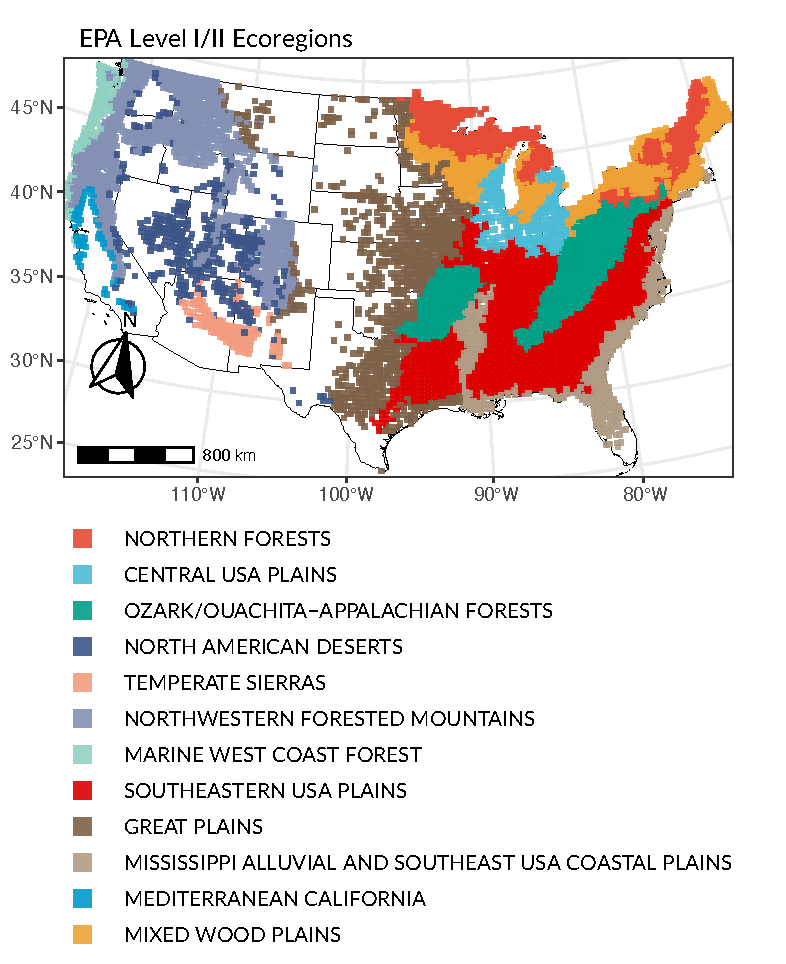
\includegraphics[width=1.1\textwidth]{../../figures/tradeoff_drivers/tradeoff_ecoregion_map.png}
\caption{\label{fig:org5003cda}Location of study grid cells within EPA level I/II ecoregions in the contiguous United States.}
\end{figure}
\subsubsection{Accounting for spatial autocorrelation}
\label{sec:org1b03438}
\begin{figure}[htbp]
\centering
\includegraphics[width=1.1\textwidth]{../../figures/tradeoff_drivers/variograms_tradeoff_drivers.png}
\caption{\label{fig:org4927791}Semivariograms depicting spatial autocorrelation in the residuals of the three meta-analytic models of tradeoff strength and adherence. Increasing trends in semivariance with distance indicate the presence of residual spatial autocorrelation. The size of points refers to the 'pair count' or numbers of unique pairs of observations used in the calculation of semivariance at that distance.}
\end{figure}

We detected evidence of significant residual spatial autocorrelation in all three models of tradeoff strength and adherence described above (Fig. \ref{fig:org4927791}). To account for this autocorrelation, which can artificially deflate estimates of parameter uncertainty, we implemented a spatial block bootstrap that resamples contiguous spatial units rather than individual observations (\cslcitation{29}{Lahiri 2018}). For each fitted model, we first estimated the characteristic scale of spatial dependence by computing an empirical variogram of model residuals and fitting a spherical variogram model. The fitted range was used to define the spatial block size. Bootstrap samples were generated by randomly selecting blocks with replacement and including all observations falling within each selected block. Blocks were located by randomly placing centerpoints within the bounding box of the full dataset. Blocks were accumulated until the bootstrap sample contained at least 95\% of the original sample size, and samples exceeding 105\% of the original size were randomly downsampled to maintain a consistent sample size. For models including categorical predictors, bootstrap samples were required to retain all factor levels present in the original data. Each bootstrap sample was refit using the same weighted regression specification as the original model. Uncertainty in model coefficients was quantified using the bootstrap distributions, with point estimates taken as the predictions of the original model and 95\% confidence intervals defined by the 2.5th and 97.5th percentiles in bootstrap samples.
\subsection{Estimating tradeoff strength relative to the regional species pool}
\label{sec:org2c3c6de}
In addition to evaluating how average tradeoff strength varies among ecoregions relative to the overall tradeoff across all species, we examined differences between community-level tradeoffs and those observed within regional species pools. This comparison provides a more direct test of community assembly, as broad geographic variation in tradeoff strength among large ecoregions may reflect processes unrelated to local competition, such as evolutionary history or environmental filtering. By contrast, comparing community-level tradeoffs to those within the regional species pool allows us to assess whether tradeoffs at the community scale are stronger than among the set of species that could realistically disperse into that community. Stronger community-level tradeoffs would therefore suggest that local competitive interactions exclude geographically proximate species that might otherwise establish.

We further evaluated how the difference between community and regional tradeoff strength varies with the spatial scale of the regional pool. This difference is expected to be small at local scales, where community and regional species pools largely overlap, and to increase as the regional pool expands. A monotonic increase in this difference—particularly if community-level tradeoffs exceed regional tradeoffs even at modest spatial scales—would provide additional evidence for the role of community assembly in shaping drought tolerance–resource acquisitiveness tradeoffs.

To generate comparisons between community- and regional-scale tradeoffs, we randomly sampled circular regions with radii ranging from 10 to 500 km. For each radius, we selected 1,000 circular regions; however, due to the irregular spatial distribution of FIA plots across the contiguous United States, some regions contained no plots, such that the number of non-empty regions considered at each radius ranged from approximately 900 to 1,000. Within each circle, tree-level data from all FIA conditions were pooled, and species abundances were aggregated by summing trees per acre (TPA) across conditions. We then estimated the slope of the tradeoff between drought tolerance and resource acquisitiveness at this regional scale using the same methodology described in the main text.

We next estimated the average community-level tradeoff slope within each region while accounting for both sampling uncertainty and between-plot heterogeneity. Let \(\beta_i\) denote the tradeoff slope estimated for plot \(i\), with variance \(\sigma_i^2\), and let \(BA_i\) be the basal area of plot \(i\). We first estimated the community-level mean tradeoff slope using inverse-variance weighting,

\[
\hat{\beta}_{\mathrm{comm}} =
\frac{\sum_i w_i \beta_i}{\sum_i w_i},
\qquad
w_i = \frac{1}{\sigma_i^2}.
\]

To quantify heterogeneity among plot-level slopes, we computed the Cochran \(Q\) statistic and estimated the between-plot variance \(\tau^2\), again using the DerSimonian--Laird method. The total variance for each plot-level estimate was then inflated as \(\sigma_i^2 + \tau^2\), yielding heterogeneity-adjusted inverse-variance weights.

We defined two normalized weight vectors over the same set of plots: (i) basal-area weights \(a_i = BA_i / \sum_j BA_j\), representing the approximate contribution of each plot to the regional estimate, and (ii) heterogeneity-adjusted inverse-variance weights \(b_i = (\sigma_i^2 + \tau^2)^{-1} / \sum_j (\sigma_j^2 + \tau^2)^{-1}\), representing the contribution of each plot to the average community-level estimator. Using these weights, we computed the variances of the regional (\(r\)) and community (\(c\)) estimators as

\[
\mathrm{Var}_{\mathrm{r}} = \sum_i a_i^2 (\sigma_i^2 + \tau^2),
\qquad
\mathrm{Var}_{\mathrm{c}} = \sum_i b_i^2 (\sigma_i^2 + \tau^2),
\]

and their covariance,

\[
\mathrm{Cov}_{\mathrm{r,c}} =
\sum_i a_i b_i (\sigma_i^2 + \tau^2),
\]

which arises because both estimators are constructed from the same underlying plot-level data. The difference between the regional and community tradeoff slopes for a given circular region was computed as \(\hat{d} = \hat{\beta}_{\mathrm{r}} - \hat{\beta}_{\mathrm{c}}\), and its uncertainty was obtained by propagating variance and covariance,

\[
\mathrm{SE}(\hat{d}) =
\sqrt{
\mathrm{Var}_{\mathrm{r}} +
\mathrm{Var}_{\mathrm{c}} -
2\,\mathrm{Cov}_{\mathrm{r,c}}
}.
\]

After quantifying \(\hat{d}\) and \(SE(\hat{d})\) for each circle of a given radius, we fit a meta-analytic model to estimate the typical difference between community-level and regional tradeoffs for that spatial scale. Finally, to evaluate how the difference in tradeoff slope between community and region varies by region size, we fit a meta-regression for the relationship between \(\hat{d}\) and the radius of the regions. All meta-analytic models were fit using the \texttt{rma} function in the \texttt{metafor} package (version 4.8-0).
\subsection{Modeling mortality response to drought}
\label{sec:org08599bc}
To assess the relationship between functional tradeoffs and mortality response to drought, we fit a zero-inflated generalized additive model of the following form:

\[
logit(\nu_i) = \alpha_0 + \sum \alpha_k x^a_{ik} + \sum_k f_k^{\nu}(x^b_{ik})
\]
\[
logit(\mu_i) = \beta_0 + \sum \beta_k z^a_{ik} \sum_k f_k^{\mu}(z^b_{ik})
\]

where \(\nu\)\textsubscript{i} is the probability that the observation, \(y_i\), is zero; \(\mu\)\textsubscript{i} \(\in\) (0,1) is the expected mortality rate given \(y_i > 0\); \(\alpha\) and \(\beta\) are linear coefficients; \(x^a_{ik}\) and \(z^a_{ik}\) are the values of linear predictor \(k\) for the Bernoulli and beta components, respectively; \(x^b_{ik}\) and \(z^b_{ik}\) are smooth predictors; and \(f_k^{\pi}(.)\) are smooth functions of predictors \(x^b_{ik}\) and \(z^b_{ik}\).

\begin{longtable}{lll}
\caption{\label{tab:org9c1582b}Mortality Model Specification}
\\
\textbf{Sub-Model} & \textbf{Linear vs. Smooth} & \textbf{Variable}\\
\hline
\endfirsthead
\multicolumn{3}{l}{Continued from previous page} \\
\hline

\textbf{Sub-Model} & \textbf{Linear vs. Smooth} & \textbf{Variable} \\

\hline
\endhead
\hline\multicolumn{3}{r}{Continued on next page} \\
\endfoot
\endlastfoot
\hline
Beta (\(\mu\)) & Linear & Tradeoff Strength\\
 &  & Tradeoff Adherence\\
 &  & CWM Drought Tol.\\
 &  & CWM Resource Acq.\\
 &  & Range Drought Tol.\\
 &  & Range Resource Acq.\\
 &  & Drought Strength\\
 &  & Drought Burden\\
 &  & Elevation\\
 &  & MAP\\
 &  & MAT\\
 &  & Stand Age\\
 &  & Basal Area\\
 &  & Drought Strength x Basal Area\\
 &  & Tradeoff Strength x Basal Area\\
 &  & Tradeoff Adherence x Basal Area\\
 & Smooth & Latitude\\
 &  & Longitude\\
 &  & Year\\
\hline
Bernoulli (\(\nu\)) & Linear & Drought Strength\\
 &  & Drought Burden\\
 &  & Elevation\\
 &  & MAP\\
 &  & MAT\\
 &  & Stand Age\\
 &  & Basal Area\\
 &  & Drought Strength x Basal Area\\
 & Smooth & Latitude\\
 &  & Longitude\\
 &  & Year\\
\hline
\end{longtable}


Because the Bernoulli and beta components of the model are specified separately, the identify of the predictors are allowed to vary. The full specification of the model can be found in Table \ref{tab:org9c1582b}. Our rationale for not including tradeoff and trait metrics in the Bernoulli component of the model was that the occurrence of positive mortality is highly stochastic, and more likely to be driven by climate, drought, and stand characteristics than competition and community assembly (\cslcitation{59}{Trugman \textit{et al.} 2021}; \cslcitation{61}{Venturas \textit{et al.} 2021}). Moreover, explaining the difference between no mortality and any mortality was of less interest than investigating the wide range of observed mortality rates which were greater than zero. 

We included three penalized beta-splines in both components of the model on each of year, latitude, and longitude. The spline on year was included to account for large-scale temporal trends and reduce temporal autocorrelation in the residuals. Likewise, the splines on latitude and longitude were designed to capture unmeasured geospatial variation across the FIA dataset, and to account for spatial autocorrelation. We allowed 3 degrees of freedom for the temporal spline, and 18 degrees of freedom for each of the spatial splines. These values were chosen to allow sufficient flexibility in capturing the underlying relationships without overfitting to small-scale trends. The model was fit using the generalized additive models for location, scale, and shape (GAMLSS) framework, which allows for substantial flexibility in modeling parametric distributions using additive smoothers. The model was fit using the 'gamlss' package (version 5.4-22) in R (\cslcitation{56}{Stasinopoulos \& Rigby 2007}), and all predictors except year, latitude and longitude were normalized to standard units to aid model fitting and facilitate the comparison of effect sizes.

To estimate a combined effect of each covariate on mortality for both inference and visualization, we calculated the expected annualized mortality rate as \((1 - \nu_i)\mu_i\). The delta method was then used to calculate approximate standard errors and confidence intervals for the combined metric (\cslcitation{42}{Oehlert 1992}). 
\subsection{Modeling growth response to drought}
\label{sec:org373c887}
\begin{longtable}{ll}
\caption{\label{tab:orgb167cc2}Growth Model Specification}
\\
\textbf{Linear vs. Smooth} & \textbf{Variable}\\
\hline
\endfirsthead
\multicolumn{2}{l}{Continued from previous page} \\
\hline

\textbf{Linear vs. Smooth} & \textbf{Variable} \\

\hline
\endhead
\hline\multicolumn{2}{r}{Continued on next page} \\
\endfoot
\endlastfoot
\hline
Linear & Tradeoff Strength\\
 & Tradeoff Adherence\\
 & CWM Drought Tol.\\
 & CWM Resource Acq.\\
 & Range Drought Tol.\\
 & Range Resource Acq.\\
 & Drought Strength\\
 & Drought Burden\\
 & Elevation\\
 & MAP\\
 & MAT\\
 & Stand Age\\
 & Basal Area\\
 & Drought Strength x Basal Area\\
 & Tradeoff Strength x Basal Area\\
 & Tradeoff Adherence x Basal Area\\
Smooth & Latitude\\
 & Longitude\\
 & Year\\
\hline
\end{longtable}

To model growth response to drought, we fit a Gaussian generalized additive model for the relationship between annualized basal area growth rate and the same list of predictors used in the beta component of the mortality model. We again included three splines on year, latitude and longitude. Here we used penalized regression splines as implemented in the 'mgcv' package in R, allowing up to 10 knots for year, and 20 knots for both latitude and longitude. Covariates were again normalized to standard units before model fitting.
\subsection{Sensitivity Analyses}
\label{sec:org0706956}
One of our primary findings is that communities that more closely adhere to tradeoffs between drought tolerance and resource acquisitiveness experience lower mortality and faster basal area growth during drought. However, interpretation of this result could be complicated by collinearity between tradeoff adherence and the range of drought tolerance and resource acquisitiveness within communities. Some degree of correlation is expected, as tradeoff adherence reflects the dispersion of traits around the tradeoff, and communities spanning a wider range of trait values may exhibit greater spread. The correlation between tradeoff adherence and the range in drought tolerance was modest (r = 0.12), whereas the correlation with the range in resource acquisitiveness was stronger (r = 0.38). To assess the robustness of our results to this collinearity, we refit the mortality and growth models under two alternative specifications: (i) excluding both trait range variables while retaining tradeoff adherence, and (ii) excluding tradeoff adherence while retaining both trait range variables.

Excluding the range variables did not qualitatively alter results for either mortality or growth (Tables \ref{tab:org890c410}, \ref{tab:org4fddf1f}). In the mortality model, the estimated effect of tradeoff adherence was nearly unchanged (0.023 [0.01, 0.037] versus 0.024 [0.012, 0.036]). In the growth model, removing the range variables strengthened the estimated effect of tradeoff adherence (-0.047 [-0.057, -0.036] versus -0.025 [-0.04, -0.01]), suggesting that tradeoff adherence absorbed part of the negative effect previously attributed to the range in resource acquisitiveness (Table \ref{tab:org73160b1}). This result supports inclusion of both tradeoff adherence and trait range metrics in the full model, as omission of either may inflate the estimated effect of the other.

Similarly, excluding tradeoff adherence had little effect on the estimated impacts of trait ranges. In mortality models, estimated effects of the range in drought tolerance (-0.005 [-0.02, 0.01] versus -0.002 [-0.017, 0.012]) and the range in resource acquisitiveness (0.005 [-0.011, 0.02] versus 0.008 [-0.005, 0.022]) were largely unchanged (Table \ref{tab:org57266e5}). The same pattern held for growth models, with minimal differences in estimated effects of drought tolerance range (-0.002 [-0.01, 0.01] versus -0.006 [-0.018, 0.006]) and resource acquisitiveness range (-0.05 [-0.06, -0.04] versus -0.049 [-0.061, -0.037]) when tradeoff adherence was excluded (Table \ref{tab:org48e4b8e}). Together, these results indicate that collinearity between trait ranges and tradeoff adherence does not explain, nor substantially influence, the observed relationships between tradeoff adherence and forest mortality or growth during drought.
\subsection{Supplementary Tables}
\label{sec:org99b7721}

\begin{longtable}{p{6.5cm}rrrr}
\caption{\label{tab:org000ebd9}Tradeoff Strength by Ecoregion}
\\
Ecoregion & n & Mean & 95\% CI (lower) & 95\% CI (upper)\\
\hline
\endfirsthead
\multicolumn{5}{l}{Continued from previous page} \\
\hline

Ecoregion & n & Mean & 95\% CI (lower) & 95\% CI (upper) \\

\hline
\endhead
\hline\multicolumn{5}{r}{Continued on next page} \\
\endfoot
\endlastfoot
\hline
Central USA Plains & 306 & -2.17 & -2.85 & -1.31\\
Great Plains & 1007 & -1.14 & -1.28 & -0.79\\
Marine West Coast Forest & 131 & -1.51 & -1.87 & -0.78\\
Mediterranean California & 61 & -0.02 & -0.20 & 0.51\\
Mississippi Alluvial And Southeast USA Coastal Plains & 493 & -0.55 & -1.06 & -0.004\\
Mixed Wood Plains & 710 & 0.58 & -2.29 & 0.69\\
North American Deserts & 431 & -1.83 & -1.83 & -1.83\\
Northern Forests & 690 & -2.50 & -2.88 & -1.87\\
Northwestern Forested Mountains & 1234 & -1.77 & -1.82 & -1.61\\
Ozark/Ouachita-Appalachian Forests & 851 & -1.99 & -2.25 & -1.71\\
Southeastern USA Plains & 1607 & -1.34 & -1.45 & -1.16\\
Temperate Sierras & 144 & -1.81 & -1.82 & -0.63\\
\end{longtable}

\begin{longtable}{lrrrr}
\caption{\label{tab:org8e088e5}Biophysical Drivers of Tradeoff Strength}
\\
Coefficient & Estimate & 95\% CI (lower) & 95\% CI (upper)\\
\hline
\endfirsthead
\multicolumn{4}{l}{Continued from previous page} \\
\hline

Coefficient & Estimate & 95\% CI (lower) & 95\% CI (upper) \\

\hline
\endhead
\hline\multicolumn{4}{r}{Continued on next page} \\
\endfoot
\endlastfoot
\hline
(Intercept) & -1.27 & -1.64 & -0.58\\
MAP & 0.18 & 0.04 & 0.53\\
MAT & 0.06 & -0.17 & 0.16\\
Stand Age & -0.01 & -0.17 & 0.02\\
\hline
\end{longtable}

\begin{longtable}{lrrr}
\caption{\label{tab:org19f703d}Biophysical Drivers of Tradeoff Adherence}
\\
Coefficient & Estimate & 95\% CI (lower) & 95\% CI (upper)\\
\hline
\endfirsthead
\multicolumn{4}{l}{Continued from previous page} \\
\hline

Coefficient & Estimate & 95\% CI (lower) & 95\% CI (upper) \\

\hline
\endhead
\hline\multicolumn{4}{r}{Continued on next page} \\
\endfoot
\endlastfoot
\hline
(Intercept) & -1.48 & -1.60 & -1.40\\
map\textsubscript{scaled} & 0.31 & 0.19 & 0.41\\
mat\textsubscript{scaled} & -0.29 & -0.38 & -0.19\\
stand\textsubscript{age}\textsubscript{scaled} & -0.14 & -0.29 & 0.05\\
\hline
\end{longtable}

\begin{longtable}{lrrrr}
\caption{\label{tab:org6fbeaae}Full Mortality Model Results}
\\
Coefficient & Estimate & Std. Error & 95\% CI (lower) & 95\% CI (upper)\\
\hline
\endfirsthead
\multicolumn{5}{l}{Continued from previous page} \\
\hline

Coefficient & Estimate & Std. Error & 95\% CI (lower) & 95\% CI (upper) \\

\hline
\endhead
\hline\multicolumn{5}{r}{Continued on next page} \\
\endfoot
\endlastfoot
\hline
\uline{\textbf{\(\mu\) component}} &  &  &  & \\
(Intercept) & -4.771 & 0.153 & -5.072 & -4.470\\
BA & -0.095 & 0.007 & -0.108 & -0.081\\
Drought Strength & -0.039 & 0.006 & -0.050 & -0.028\\
Drought Burden & 0.046 & 0.007 & 0.032 & 0.059\\
Tradeoff Strength & 0.006 & 0.007 & -0.007 & 0.019\\
Tradeoff Adherence & 0.023 & 0.007 & 0.010 & 0.037\\
MAP & 0.119 & 0.007 & 0.106 & 0.132\\
MAT & 0.022 & 0.027 & -0.032 & 0.077\\
CWM Drought Tol. & -0.025 & 0.008 & -0.042 & -0.009\\
CWM Resource Acq. & 0.019 & 0.008 & 0.004 & 0.034\\
Range Drought Tol. & -0.005 & 0.008 & -0.020 & 0.010\\
Range Resource Acq. & 0.005 & 0.008 & -0.011 & 0.020\\
Elevation & 0.028 & 0.014 & 0.000 & 0.056\\
Stand Age & 0.022 & 0.007 & 0.009 & 0.035\\
BA x Drought Strength & -0.008 & 0.006 & -0.021 & 0.004\\
BA x Tradeoff Strength & -0.003 & 0.006 & -0.014 & 0.009\\
BA x Tradeoff Adherence & 0.002 & 0.006 & -0.010 & 0.014\\
\hline
\uline{\textbf{\(\nu\) component}} &  &  &  & \\
(Intercept) & -6.255 & 0.323 & -6.892 & -5.618\\
BA & -0.260 & 0.013 & -0.287 & -0.234\\
Drought Strength & 0.074 & 0.013 & 0.048 & 0.100\\
Drought Burden & 0.020 & 0.014 & -0.008 & 0.049\\
MAP & -0.010 & 0.015 & -0.039 & 0.019\\
MAT & 0.658 & 0.060 & 0.540 & 0.776\\
Elevation & -0.174 & 0.030 & -0.234 & -0.114\\
Stand Age & -0.075 & 0.015 & -0.104 & -0.046\\
BA x Drought Strength & 0.031 & 0.014 & 0.004 & 0.058\\
\hline
\end{longtable}

\begin{longtable}{lrrrr}
\caption{\label{tab:org73160b1}Full Growth Model Results}
\\
Coefficient & Estimate & Std. Error & 95\% CI (lower) & 95\% CI (upper)\\
\hline
\endfirsthead
\multicolumn{5}{l}{Continued from previous page} \\
\hline

Coefficient & Estimate & Std. Error & 95\% CI (lower) & 95\% CI (upper) \\

\hline
\endhead
\hline\multicolumn{5}{r}{Continued on next page} \\
\endfoot
\endlastfoot
\hline
(Intercept) & -0.173 & 0.022 & -0.22 & -0.13\\
BA & -0.260 & 0.006 & -0.27 & -0.25\\
Drought Strength & 0.035 & 0.006 & 0.02 & 0.05\\
Drought Burden & 0.014 & 0.007 & 0.00 & 0.03\\
Tradeoff Strength & -0.018 & 0.006 & -0.03 & -0.01\\
Tradeoff Adherence & -0.025 & 0.006 & -0.04 & -0.01\\
MAP & 0.119 & 0.008 & 0.10 & 0.14\\
MAT & -0.027 & 0.031 & -0.09 & 0.03\\
CWM Drought Tol. & -0.007 & 0.007 & -0.02 & 0.01\\
CWM Resource Acq. & -0.026 & 0.008 & -0.04 & -0.01\\
Range Drought Tol. & -0.002 & 0.006 & -0.01 & 0.01\\
Range Resource Acq. & -0.050 & 0.007 & -0.06 & -0.04\\
Elevation & -0.038 & 0.021 & -0.08 & 0.00\\
Stand Age & -0.197 & 0.006 & -0.21 & -0.19\\
BA x Drought Strength & 0.077 & 0.005 & 0.07 & 0.09\\
BA x Tradeoff Strength & -0.001 & 0.005 & -0.01 & 0.01\\
BA x Tradeoff Adherence & -0.023 & 0.005 & -0.03 & -0.01\\
\hline
\end{longtable}

\begin{longtable}{lrrrr}
\caption{\label{tab:org890c410}Mortality Model (without trait range variables)}
\\
Coefficient & Estimate & Std. Error & 95\% CI (lower) & 95\% CI (upper)\\
\hline
\endfirsthead
\multicolumn{5}{l}{Continued from previous page} \\
\hline

Coefficient & Estimate & Std. Error & 95\% CI (lower) & 95\% CI (upper) \\

\hline
\endhead
\hline\multicolumn{5}{r}{Continued on next page} \\
\endfoot
\endlastfoot
\hline
\uline{\textbf{\(\mu\) component}} &  &  &  & \\
(Intercept) & -4.762 & 0.150 & -5.059 & -4.466\\
PB(year) & 0.006 & 0.001 & 0.004 & 0.008\\
PB(lon) & 0.005 & 0.001 & 0.003 & 0.006\\
PB(lat) & 0.014 & 0.005 & 0.005 & 0.023\\
BA & -0.095 & 0.007 & -0.108 & -0.081\\
Drought Strength & -0.039 & 0.006 & -0.050 & -0.028\\
Drought Burden & 0.046 & 0.007 & 0.032 & 0.059\\
Tradeoff Strength & 0.004 & 0.006 & -0.008 & 0.015\\
Tradeoff Adherence & 0.024 & 0.006 & 0.012 & 0.036\\
MAP & 0.119 & 0.007 & 0.106 & 0.133\\
MAT & 0.022 & 0.027 & -0.032 & 0.075\\
CWM Drought Tol. & -0.027 & 0.007 & -0.041 & -0.013\\
CWM Resource Acq. & 0.019 & 0.008 & 0.004 & 0.034\\
Elevation & 0.029 & 0.014 & 0.001 & 0.057\\
Stand Age & 0.022 & 0.007 & 0.009 & 0.035\\
BA x Drought Strength & -0.008 & 0.006 & -0.021 & 0.004\\
BA x Tradeoff Strength & -0.003 & 0.006 & -0.014 & 0.008\\
BA x Tradeoff Adherence & 0.002 & 0.006 & -0.009 & 0.014\\
\hline
\uline{\textbf{\(\nu\) component}} &  &  &  & \\
(Intercept) & -6.261 & 0.323 & -6.898 & -5.625\\
PB(year) & -0.030 & 0.002 & -0.035 & -0.026\\
PB(lon) & -0.035 & 0.001 & -0.038 & -0.032\\
PB(lat) & 0.056 & 0.010 & 0.036 & 0.076\\
BA & -0.260 & 0.013 & -0.286 & -0.233\\
Drought Strength & 0.075 & 0.013 & 0.049 & 0.101\\
Drought Burden & 0.021 & 0.014 & -0.007 & 0.049\\
MAP & -0.010 & 0.015 & -0.039 & 0.019\\
MAT & 0.660 & 0.060 & 0.541 & 0.778\\
Elevation & -0.172 & 0.030 & -0.232 & -0.112\\
Stand Age & -0.075 & 0.015 & -0.104 & -0.046\\
BA x Drought Strength & 0.031 & 0.014 & 0.005 & 0.058\\
\hline
\end{longtable}

\begin{longtable}{lrrrr}
\caption{\label{tab:org57266e5}Mortality Model (no tradeoff variables)}
\\
Coefficient & Estimate & Std. Error & 95\% CI (lower) & 95\% CI (upper)\\
\hline
\endfirsthead
\multicolumn{5}{l}{Continued from previous page} \\
\hline

Coefficient & Estimate & Std. Error & 95\% CI (lower) & 95\% CI (upper) \\

\hline
\endhead
\hline\multicolumn{5}{r}{Continued on next page} \\
\endfoot
\endlastfoot
\hline
\uline{\textbf{\(\mu\) component}} &  &  &  & \\
(Intercept) & -4.704 & 0.152 & -5.003 & -4.404\\
BA & -0.096 & 0.007 & -0.109 & -0.083\\
Drought Strength & -0.039 & 0.006 & -0.050 & -0.028\\
Drought Burden & 0.046 & 0.007 & 0.033 & 0.060\\
MAP & 0.117 & 0.007 & 0.104 & 0.130\\
MAT & 0.021 & 0.027 & -0.033 & 0.075\\
CWM Drought Tol. & -0.029 & 0.008 & -0.045 & -0.013\\
CWM Resource Acq. & 0.018 & 0.008 & 0.003 & 0.033\\
Range Drought Tol. & -0.002 & 0.007 & -0.017 & 0.012\\
Range Resource Acq. & 0.008 & 0.007 & -0.005 & 0.022\\
Elevation & 0.029 & 0.014 & 0.002 & 0.057\\
Stand Age & 0.022 & 0.007 & 0.009 & 0.036\\
BA x Drought Strength & -0.009 & 0.006 & -0.021 & 0.003\\
\hline
\uline{\textbf{\(\nu\) component}} &  &  &  & \\
(Intercept) & -6.261 & 0.323 & -6.898 & -5.625\\
BA & -0.260 & 0.013 & -0.286 & -0.233\\
Drought Strength & 0.075 & 0.013 & 0.049 & 0.101\\
Drought Burden & 0.021 & 0.014 & -0.007 & 0.049\\
MAP & -0.010 & 0.015 & -0.039 & 0.019\\
MAT & 0.660 & 0.060 & 0.541 & 0.778\\
Elevation & -0.172 & 0.030 & -0.232 & -0.112\\
Stand Age & -0.075 & 0.015 & -0.104 & -0.046\\
BA x Drought Strength & 0.031 & 0.014 & 0.005 & 0.058\\
\hline
\end{longtable}

\begin{longtable}{lrrrr}
\caption{\label{tab:org4fddf1f}Growth model (without trait range variables)}
\\
Coefficient & Estimate & Std. Error & 95\% CI (lower) & 95\% CI (upper)\\
\hline
\endfirsthead
\multicolumn{5}{l}{Continued from previous page} \\
\hline

Coefficient & Estimate & Std. Error & 95\% CI (lower) & 95\% CI (upper) \\

\hline
\endhead
\hline\multicolumn{5}{r}{Continued on next page} \\
\endfoot
\endlastfoot
\hline
(Intercept) & -0.173 & 0.023 & -0.218 & -0.128\\
BA & -0.261 & 0.006 & -0.272 & -0.250\\
Drought Strength & 0.035 & 0.006 & 0.024 & 0.046\\
Drought Burden & 0.014 & 0.007 & 0.000 & 0.027\\
Tradeoff Strength & 0.003 & 0.005 & -0.007 & 0.014\\
Tradeoff Adherence & -0.047 & 0.005 & -0.057 & -0.036\\
MAP & 0.121 & 0.008 & 0.104 & 0.138\\
MAT & -0.019 & 0.031 & -0.079 & 0.042\\
CWM Drought Tol. & -0.013 & 0.006 & -0.026 & -0.001\\
CWM Resource Acq. & -0.026 & 0.008 & -0.042 & -0.010\\
Elevation & -0.038 & 0.021 & -0.079 & 0.003\\
Stand Age & -0.197 & 0.006 & -0.209 & -0.186\\
BA x Drought Strength & 0.077 & 0.005 & 0.067 & 0.087\\
BA x Tradeoff Strength & 0.000 & 0.005 & -0.009 & 0.009\\
BA x Tradeoff Adherence & -0.023 & 0.005 & -0.033 & -0.014\\
\hline
\end{longtable}

\begin{longtable}{lrrrr}
\caption{\label{tab:org48e4b8e}Growth Model (without tradeoff variables)}
\\
Coefficient & Estimate & Std. Error & 95\% CI (lower) & 95\% CI (upper)\\
\hline
\endfirsthead
\multicolumn{5}{l}{Continued from previous page} \\
\hline

Coefficient & Estimate & Std. Error & 95\% CI (lower) & 95\% CI (upper) \\

\hline
\endhead
\hline\multicolumn{5}{r}{Continued on next page} \\
\endfoot
\endlastfoot
\hline
(Intercept) & -0.158 & 0.021 & -0.199 & -0.116\\
BA & -0.252 & 0.005 & -0.263 & -0.242\\
Drought Strength & 0.034 & 0.006 & 0.023 & 0.045\\
Drought Burden & 0.013 & 0.007 & 0.000 & 0.027\\
MAP & 0.127 & 0.008 & 0.110 & 0.143\\
MAT & -0.028 & 0.031 & -0.089 & 0.032\\
CWM Drought Tol. & -0.002 & 0.007 & -0.015 & 0.011\\
CWM Resource Acq. & -0.024 & 0.008 & -0.040 & -0.008\\
Range Drought Tol. & -0.006 & 0.006 & -0.018 & 0.006\\
Range Resource Acq. & -0.049 & 0.006 & -0.061 & -0.037\\
Elevation & -0.042 & 0.021 & -0.083 & -0.001\\
Stand Age & -0.197 & 0.006 & -0.208 & -0.186\\
BA x Drought Strength & 0.081 & 0.005 & 0.070 & 0.091\\
\hline
\end{longtable}
\end{document}
